%%% Local Variables:
%%% coding: utf-8
%%% mode: latex
%%% TeX-master: t
%%% End:
%
% -----------------------------------------------------------------------------
%  Kochbuch - Moppels Rezeptsammlung                          % vim:sw=2:ts=2
% -----------------------------------------------------------------------------
%
% general document setup
\documentclass[
	12pt,
	a4paper,
	titlepage,
	oneside]{book}
  \usepackage{kochbuch}
  \hypersetup{
    pdftitle={Moppels Rezeptsammlung},
    pdfsubject={Inspiriert von verschiedenen Sterneköchen},
    pdfauthor={Lutz Moppert},
    pdfkeywords = {Stichwort1, Stichwort2 ...} ,
    pdfcreator  = {pdflatex},
    }
%
% -----------------------------------------------------------------------------
%  Document colors
%
% Colors for title page
\colorlet{SubjectColor}{LimeGreen}
\colorlet{TitleColor}{LimeGreen}
\colorlet{SubtitleColor}{LimeGreen}
\colorlet{AuthorColor}{LimeGreen}
\colorlet{DateColor}{LimeGreen}

% Color for Recipes
\colorlet{ChapterColor}{OliveGreen}
\colorlet{RecipeColor}{OliveGreen}
\colorlet{IngredientColor}{OliveGreen}
\colorlet{LetterColor}{OliveGreen}

% Layout Colors
\colorlet{PageNumberColor}{MidnightBlue}
\colorlet{PageHeadFootColor}{MidnightBlue}
\colorlet{IndexHeadingColor}{MidnightBlue}

% Set general font for document
\usepackage[sfdefault,light]{roboto}

%
%  Ende der Preambel
% -----------------------------------------------------------------------------
%
\begin{document}
%
% -----------------------------------------------------------------------------
%  Titelseite
%
\frontmatter
\begin{titlepage}
\begin{center}
  \vspace*{4cm}
  \Huge{\textbf{Cooking}} \\[15pt]
  \LARGE{How to do it, and survive} \\
 % ----------------------------------------------------------------
  \vspace{1.5cm}
  \large{Author}\\[5pt]
  \Large{\textbf{Author Name}} \\
  \vfill
 % ----------------------------------------------------------------
  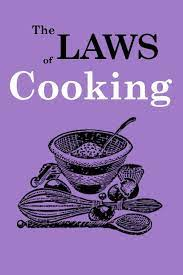
\includegraphics[width=0.35\textwidth]{Bilder/title.jpg}\\[5pt]
  \vspace{1cm}
  {January 2022}
\end{center}
\end{titlepage}

\newpage

% Table of contents
\tableofcontents
%
% -----------------------------------------------------------------------------
%  Kapitel
%
\mainmatter

\category[Bilder/Gericht.jpg]{Gerichte}

\category[Bilder/Grundlage.jpg]{Grundlagen}
  \begin{recipe}{Hollandaise}{nach Dieter Müller}
  \label{Hollandaise}
  \inglist
  \ingredient{150 g Butter}
  \ingredient{3 Eigelb}
  \ingredient{3 EL kaltes Wasser}
  \ingredient{1 EL Weißwein}
  \ingredient{Saft von \halb Zitrone}
  
  \steps
  Die Butter bei milder Hitze zerlassen. In eine Topf die Eigelb mit dem Wasser und dem
  Wein verrühren und im Wasserbad cremig aufschlagen. Anschließend die zerlassene Butter
  langsam unterrühren.

  Die Sauce im Wasserbad weiter schlagen, bis sie cremig ist, mit Salz und Zitronensaft 
  abschmecken und \textit{sofort} servieren.
  
  Mit 2-3 Eßlöffeln geschlagener Sahne wird aus der Hollandaise eine Mousseline, die sich
  hervoragend zum gratinieren eignet.
\end{recipe}

  \begin{recipe}{Bearnaise}{nach Dieter Müller}
  \label{Bearnaise}
  \inglist
  \ingredient{2 TL Estragonessig}
  \ingredient{1 EL Estragonblätter}
  \ingredient{1 EL Petersilie}
  \ingredient{1-2 Schalotten}
  \ingredient{100 ml Weißwein}
  \ingredient{Zitronensaft}
  
  \steps
  Die Kräuter und die Schalotten fein hacken und mit dem Weißwein und etwas Zitronensaft
  in einen Topf geben. Mit Salz und Pfeffer würzen und das ganze stark einreduzieren, bis
  fast alle Flüssigkeit verdampft ist.

  Die Reduktion wird in die Sauce Hollandaise (siehe Seite \pageref{Hollandaise}) gegeben 
  und passt gut zu gebratenem Fleisch.
\end{recipe}



  \begin{recipe}{Mayonnaise}{nach Kolja Kleeberg}
  \label{Mayonnaise}
  \inglist
  \ingredient{1 Ei}
  \ingredient{1 TL Senf}
  \ingredient{1 spritzer Zitronensaft}
  \ingredient{100 ml Öl}
  
  \steps
  Alle Zutaten in einen hohen schmalen Becher füllen, den Mixstab hineinstellen,
  einschalten und langsam hochziehen.  
  
  \textbf{Tipp:} Mayonnaise immer zum Schluss noch einmal abschmecken.
  
\end{recipe}



  \newpage
  \begin{recipe}{Fisch-Weißweinsauce}{frei nach Dieter Müller}
  \label{Fischsauce}
  \inglist
  \ingredient{500 ml Fond}
  \ingredient{200 ml Weißwein}
  \ingredient{20 ml Nolly Prat}
  \ingredient{1 EL Mehlbutter}
  \ingredient{150 g Sahne}
  \ingredient{10 g Creme Fraiche}
  \ingredient{Zitronensaft}
  
  \steps
  Nolly Prat und Weißwein einreduzieren und kurz flambieren. Den Fond zugeben und alles
  auf die Hälfte reduzieren. Sahne und Creme Fraiche hinzu und nochmals auf ein Drittel
  reduzieren. Mit Zitronensaft, Fischsauce und Salz abschmecken.
\end{recipe}

  \begin{recipe}{Parmesan Espuma}{von iSi}
  \label{Parmesan Espuma}
  \inglist
  
  \ingredient{300 ml Milch}
  \ingredient{100 ml Sahne}
  \ingredient{200 g Parmesan}
  \ingredient{1 g Salz}
  \ingredient{1 g Pfeffer}

  \steps
  Milch erhitzen, Parmesan zugeben und ca. 20 Min. ziehen lassen. Sahne
  zugeben, mit Salz und Pfeffer abschmecken. Durch ein Sieb in ein 0,5 l
  Sahnespender füllen, 1 Sahnekapsel aufschrauben und kräftig schütteln.  Im
  Kühlschrank mind. 6 Stunden kühlen.

\end{recipe}

\begin{recipe}{Ziegenkäse Espuma}{von iSi}
  \label{Ziegenkäse Espuma}
  \inglist
  \ingredient{250 g Ziegenkäse mit Kräutern}
  \ingredient{125 g Sauerrahm}
  \ingredient{125 ml Sahne}
  \ingredient{45 ml Olivenöl}
  \ingredient{1 g Salz}
  \ingredient{1 g Pfeffer}
  \ingredient{1 g Zucker}


  \steps
  Ziegenkäse, Olivenöl, Sauerrahm und Gewürze in einem Standmixer fein pürieren
  und durch ein Sieb passieren. Die Sahne unterrühren, sodass die Masse eine
  kompakte Konsistenz hat. In einen 0,5 l Sahnespender füllen, 1 Sahnekapsel
  aufschrauben und kräftig schütteln. Im Kühlschrank 1-2 Stunden kühlen. 

\end{recipe}

  \newpage
  \begin{recipe}{Gefl"ugelfond}{Grundlage}
  \label{Geflügelfond}
  \inglist
  \ingredient{1,5 kg Suppenhuhn\index{Suppenhuhn}}
  \ingredient{200 ml Weißwein\index{Wei"swein}}
  \ingredient{1 Zwiebel}
  \ingredient{1 Karotte}
  \ingredient{1 Sück Knollensellerie}
  \ingredient{\halb Lauchstange}
  \ingredient{1 Knoblauchzehe}
  \ingredient{1 Lorbeerblatt}
  \ingredient{1 Thymianzweig}
  \ingredient{1 Nelke}
  \ingredient{2 Petersilienzweige}
  \ingredient{10 Pfefferkörner}

  \steps
  Das Suppenhuhn gründlich waschen, in einem großen Topf mit kaltem Wassser bedecken und
  langsam zum kochen bringen. Das Huhn 1 Stunde leise sieden lassen.

  Zwiebeln, Karotten, Knoblauch und Sellerie schälen und grob zerkleinern. Zusammen mit den
  Gewürzen in den Topf geben und das ganlze eine weitere Stunde sieden lassen.

  Den Fond durch ein Sieb passieren und erkalten lassen. Das Fleisch von Huhn kann für ein
  anderes Gericht verwendet werden, am besten als Frikasssee oder mit Majonaise, das es
  durch das kochen ein wenig trocken geworden ist.

  Um einen \textbf{dunklen Geflügelfond} herzustellen, die Knochen vom Huhn zuvor eine
  Stunde im Ofen bei ca. 150 \celsius rösten. Das zerkleinerte Gemüse im Topf anrösten,
  Tomatenmark zu geben und kurz mitrösten und erst dann zur Brühe zugeben.
\end{recipe}

  \begin{recipe}{Knoblauchcreme}{nach Elmar}
  \label{Knoblauchcreme}
  \inglist
  \ingredient{2 Philadelphia}
  \ingredient{2-3 Zehen Knoblauch}
  \ingredient{Paprikapulver}
  \ingredient{200ml geschlagene Sahne}

  \steps
  Den Knoblauch in den Frischkäse pressen, mit dem Paprikapulver würzen cremig
  schlagen. Mit Salz und Pfeffer kräftig abschmecken und schließlich die
  geschlagene Sahne vorsichtig unterheben.

\end{recipe}

  \newpage
  \begin{recipe}{Currysauce}{von Uta}
  \label{Currysauce}
  \inglist
  \ingredient{\halb Tasse Mayonaise}
  \ingredient{\halb Tasse Sahne}
  \ingredient{2 EL Tomatenketchup}
  \ingredient{4 TL Currypulver}
  \ingredient{1 EL Zitronensaft}
  \steps
  Alle Zutaten verrühren und das Ganze kalt stellen.
\end{recipe}
  \begin{recipe}{Apfel-Currycreme}{von Uta}
  \label{Apfel-Currycreme}
  \inglist
  \ingredient{1 Pckg. Frischkäse}
  \ingredient{1 Apfel}
  \ingredient{2 Frühlingszwiebeln}
  \ingredient{1 TL Currypulver}
  \ingredient{1 EL Zitronensaft}

  \steps
  Den Apfel grob reiben und die Frühlingszwiebeln in feine Ringe schneiden.
  Alle Zutaten verrühren und mit Salz und Pfeffer abschmecken. Das Ganze kalt
  stellen.
\end{recipe}

  \begin{recipe}{Erdnusssauce}{für Hähnchen}
  \inglist
  \ingredient{8 EL Chilisauce}
  \ingredient{4 EL Erdnussbutter}
  \ingredient{1 EL Sojasauce}
  \ingredient{7 EL (Kokos-)Milch}

  \steps
  Die Zutaten vermengen. Zunächst nur etwas Milch verwenden und dann nach und
  nach weitere Milch zugeben, bis die Konsistenz passt.
\end{recipe}

  \newpage
  \begin{recipe}{Hoisin}{aus dem Netz}\label{Hoisin}
  \inglist
  \ingredient{100 g Pflaumenmus}
  \ingredient{100 g Mangochutney}
  \ingredient{2 EL Sojasauce}
  \ingredient{1 EL Ingwersaft}
  \ingredient{2 EL Honig}
  \ingredient{1 EL Essig}
  \ingredient{1 TL Chilipulver}

  \steps
  Pflaumenmus und Mangochutney unter Rühren erhitzen und mit den restlichen
  Zutaten mischen. Abschließend mit dem Chilipulver abschmecken.
\end{recipe}

  \begin{recipe}{Grillmarinade}{für Hähnchen}
  \label{Marinade}
  \inglist
  \ingredient{1 EL Honig}
  \ingredient{3 EL Olivenöl}
  \ingredient{3 EL Sojasauce}
  \ingredient{3 EL Weißwein}
  \ingredient{1 EL Balsamico}
  \ingredient{1 EL Zitronensaft}
  \ingredient{1 TL Senf}
  \ingredient{2 TL Tomatenmark}
  \ingredient{1 TL Rosmarin}
  \ingredient{1 TL Oregano}
  \ingredient{1 TL Pfeffer}
  \ingredient{1 TL Paprikapulver}
  \ingredient{1 Prise Zimt}
  \ingredient{2 Knoblauchzehen}
  \ingredient{2 Chilischoten}

  \steps
  Den Knoblauch zerdrücken und die Kräuter fein hacken. Alle Zutaten vermischen
  und zu einer dickflüssigen Marinade rühren. Das Fleisch, am besten über Nacht,
  mit der Marinade bestrichen ziehen lassen. Je nach Geschmack noch ein wenig
  Salzen und dann vorsichtig grillen (der Honig verbrennt leicht).

  Wenn keine frischen Kräuter zu bekommen sind, kann man auch getrocknete
  nehmen. Diese dann am besten im Mörser ein wenig zerkleinern.
\end{recipe}

\category[Bilder/Suppe.jpg]{Suppen \& Eintöpfe}
  \begin{recipe}{Chili Con Carne}{nach Lutz Moppert}
  \inglist
  \ingredient{500 g Gehacktes\index{Fleisch>Gehacktes}\index{Hackfleisch}}
  \ingredient{1 große Zwiebel}
  \ingredient{1 EL Olivenöl}
  \ingredient{1 EL Tomatenmark}
  \ingredient{100 ml Rotwein}
  \ingredient{2 Zehen Knoblauch}
  \ingredient{2 Paprika\index{Gem"use>Paprika}}
  \ingredient{1 gr. Dose Tomaten\index{Gem"use>Tomaten}}
  \ingredient{1 kl. Dosen Kidney Bohnen\index{Gem"use>Bohnen}\index{Bohnen>Kidney}}
  \ingredient{2 getrocknete Chili}
  \ingredient{2 Lorbeerblätter}
  \ingredient{\halb TL Zucker}
  \ingredient{\halb TL Kreuzkümmel}
  \ingredient{1 TL Oregano}
  
  \steps
  Das Gehackte anbraten bis alle Flüßigkeit verdampft und das Fleisch leicht gebräunt ist.
  Dann die Zwiebel dazu geben und kurz andünsten. 
  
  Das Tomatenmark und ein wenig Olivenöl unterrühren und kurz anrösten, dann mit Rotwein
  ablöschen und wieder warten, bis die gesamte Flüßigkeit verdunstet ist. Erst jetzt die
  Tomaten zufügen und Alles eine gute Stunde köcheln lassen.
  
  Die Paprika schälen, klein schneiden, die Kidney Bohnen abtropfe und beides zu dem Sugo
  geben. Den Knoblauch in feine Scheiben schneiden und zusammen mit den restlichen
  Gewürzen ebenfalls beifügen. 
  
  Nach ca. 10 Minuten das Lorbeerblatt wieder entfernen, mit Salz und Pfeffer abschmecken
  und zur Milderung der Schärfe nach belieben mit Joghurt und Baguette servieren.
\end{recipe}

  \begin{recipe}{Serbische Bohnensuppe}{aus der Konserve}
  \inglist
  \ingredient{1 Dose Bohnen\index{Gem"use>Bohnen}\index{Bohnen>Wei"se}}
  \ingredient{1 Dose Tomaten}
  \ingredient{\halb l Brühe}
  \ingredient{\halb TL Thymian}
  \ingredient{\halb TL Oregano}
  \ingredient{\halb TL Bohnenkraut}
  \ingredient{\halb TL Estragon}
  \ingredient{\halb TL Majoran}
  \ingredient{\halb TL Selleriesalz}
  \ingredient{1 TL Paprika edelsüß}
  \ingredient{1 Knoblauchzehe}
  \ingredient{1 Peperoni}
  \ingredient{100 g Speck}
  \ingredient{25 g Butter}
  \ingredient{250 ml Sahne}
  \ingredient{2 EL Speisestärke}
  \ingredient{2 - 3 Bockwürstchen}
  \index{Suppe>Serbische Bohnensuppe}
  
  \steps
  Die Brühe mit den Gewürzen aufkochen. Den Knoblauch schälen und mit den Peperoni fein hacken und in die Brühe geben. Die Tomaten klein schneiden und \halb Stunde mitkochen, dann die Bohnen ebenfalls hinzufügen.

  Den Speck würfeln und in der Butter auslassen. Das ganze zur Suppe geben. Die Sahne mit dem Mondamin verrühren und in die Suppe geben. Das ganze aufkochen und je nach Geschmack Bockwürstchen klein schneiden und in die Suppe geben.
\end{recipe}

  \begin{recipe}{Erbsensuppe}{nach Mälzer / Witzigmann}
  \label{Erbsensuppe}
  \inglist[Zutaten]
  \inglist
  \ingredient{1 Bund Suppengrün}
  \ingredient{250 g Kartoffeln}
  \ingredient{500 g Schälerbsen}
  \ingredient{300 g durchwachsener Speck}
  \ingredient{1 Lorbeerblatt}
  \ingredient{3 Pimentkörner}
  \ingredient{2 l Brühe}
  \ingredient{2 EL Rotweinessig}
  \ingredient{Wiener Würstchen}
  \ingredient{2 Stängel Majoran}
  \ingredient{1 Bund Petersilie}
  
  \steps
  Suppengrün würfeln, Kartoffeln schälen und würfeln. Erbsen abspülen und
  abtropfen lassen. Speck würfeln und in einem großen Topf anbraten.
  Suppengrün, Kartoffeln, Lorbeer und das zerstoßene Piment zugeben und kurz
  mitbraten.

  Mit der Brühe ablöschen, dann die Erbsen dazu und das ganze mit Salz und
  Pfeffer würzen. Anschlißend gut 2 Stunden garen und dabei gelegentlich
  umrühren.

  Am Ende mit Essig abschmecken, die Würstchen in der Suppe erwärmen und mit
  dem Majoran und der Petersilie verfeinern.
\end{recipe}

  \begin{recipe}{Kartoffelsuppe}{frei nach Alfons Schuhbeck}
  \inglist
  \ingredient{700 g Kartoffeln}
  \ingredient{100 g Karotten}
  \ingredient{100 g Knollensellerie}
  \ingredient{\halb l Geflügelfond}
  \ingredient{100 ml Sahne}
  \ingredient{50 g Schimmelkäse (mild)}
  \ingredient{1 getrocknete Chili}
  \ingredient{1 Lorbeerblatt}
  \ingredient{1 Zweig Bohnenkraut}
  \ingredient{\halb TL Kreuzkümmel}
  \ingredient{\halb TL Paprikapulver}
  \index{Gem"use>Kartoffeln}
  
  \steps
  Die Kartoffeln, die Karotten und den Sellerie putzen, schälen und in 1 cm große Würfel
  schneiden. Die Gemüsewürfel mit der Brühe in einen Topf geben, das Lorbeerblatt und die
  Chili hinzufügen und zum kochen bringen. Das Gemüse anschließend knapp unter dem
  Siedpunkt etwa 20 Minuten weich garen.

  Am Ende der Garzeitdas Lorbeerblatt und die Chili wieder entffernen, ein viertel der
  Gemüsewprfel mit dem Schaumlöffel herausnehmen und beiseite stellen. Die Sahne in die
  Suppe geben, nochmals aufkochen und die restlichen Gewürze beifügen.

  Den Käse etwas zerkleinern und in der Suppe zerschmelzen lassen. Das ganze mit dem
  Stabmixer pürieren und mit Salz und Bohnenkraut abschmecken. Dann die Gemüsewürfel
  wieder in die Suppe geben und nach belieben noch Würstchen hinzufügen.
\end{recipe}



  \newpage
  \begin{recipe}{Kartoffelpilzsuppe}{frei nach Alfred Biolek}
  \inglist
  \ingredient{700 g Kartoffeln}
  \ingredient{2 Stangen Lauch}
  \ingredient{2 Frühlingszwiebeln}
  \ingredient{1 Kohlrabi}
  \ingredient{4 Karotten}
  \ingredient{100 g Butter}
  \ingredient{800 ml Wasser}
  \ingredient{1 Lorbeerblatt}
  \ingredient{1 Zweig Thymian}
  \ingredient{5 g getrocknete Steinpilze}
  \ingredient{1 Päckchen Sahne}
  \ingredient{1 Becher Creme Fra\^{\i}che}
  \index{Gem"use>Kartoffeln}

  \steps
  Die Kartoffeln schälen, waschen und in kleine Würfel schneiden. Lauch und
  Frühlingszwiebeln putzen und in schmale Ringe schneiden. Kohlrabi und
  Karotten schälen und in feine Streifen schneiden.

  Die Hälfte des Lauchs mit den Frühlingszwiebeln und den Kartoffeln in 1 EL
  Butter im Topf anschwitzen, mit dem Wasser ablöschen. Mit Salz, Pfeffer und
  Muskatnuss würzen. Thymian und Lorbeerblatt in einem Gewürzbeutel hinzugeben
  und ca. \halb Stunde köcheln lassen.

  Die Kohlrabi, Karotten und den Rest Lauch in einer Pfanne mit etwas
  Öl anbraten, dann mit ein wenig Wasser ablöschen und in 5 Minuten "`al
  dente"' dünsten. Die Steinpilze mit der Sahne im Topf aufkochen und pürieren.

  Am Ende der Garzeit den Gewürzbeutel aus der Suppe nehmen, alles pürieren.
  Creme Fra\^{\i}che und die Pilzsahne hinzugeben und nochmals pürieren. Am
  Ende das Gemüse unterrühren und evtl. mit Croutons servieren.
\end{recipe}

  \begin{recipe}{Sauerampfersuppe}{Eingenkreation}
  \inglist
  \ingredient{3 Bund Sauerampfer}
  \ingredient{2 Kartoffeln}
  \ingredient{700 ml Geflügelfond}
  \ingredient{50 g geklärte Butter}
  \ingredient{1 Becher Crème Fraîche}
  \index{Suppe>Sauerampfer}
  \index{Gem"use>Sauerampfer}

  \steps
  Vom Sauerampfer die groben Stiele entfernen, gründlich waschen und in Streifen
  schneiden. Die geklärte Butter in einem Topf erhitzen und die Gemüsestreifen darin
  zerfallen lassen.

  Den Fond zugiessen, die Kartoffeln schälen und in dünne scheiben schneiden und in die
  Suppe geben. Das Ganze ca. 30 min. simmern lassen.

  Anschließend die Suppe pürieren, die Crème Fraîche einrühren und mit Salz und Pfeffer
  abschmecken.
\end{recipe}

  \newpage
  \begin{recipe}{Kürbis-Suppe}{frei nach Schuhbeck und Lafer}
  \inglist
  \ingredient{500 g Muskat-Kürbis}
  \ingredient{2 Zwiebeln}
  \ingredient{1 Petersilienwurzel}
  \ingredient{750 ml Gemüsefond}
  \ingredient{150 ml Sahne}
  \ingredient{100 ml Kokosmilch}
  \ingredient{1 Knoblauchzehe}
  \ingredient{1 TL Currypulver}
  \ingredient{Chilipulver}
  \ingredient{1 Splitter Zimtrinde}
  \ingredient{\halb ausgekratzte Vanilleschote}
  \ingredient{40 g kalte Butter}
  \index{Gem"use>K"urbis}
  \index{Suppe>K"urbis}

  \steps
  Den Kürbis waschen, entkernen, schälen und in Würfel schneiden. Die Zwiebel und die
  Petersilienwurzel schälen und fein Würfeln. Etwas Rapsöl in einem Topf erhitzen und das
  Wurzelgemüse darin andünsten.

  Die Kürbiswürfel zugeben und das Ganze weitere 3 Minuten andünsten, dann mit dem Fond
  ablöschen, Sahne und Kokosmilch zugeben, aufkochen und bei milder Hitze 15 - 20 Minuten
  köcheln lassen

  Die Suppe mit dem Curry- und dem Chili-Pulver würzen, pürieren und durch ein Sieb
  passieren. Dann die Knoblauchzehe, Zimtrinde und die Vanilleschote in die Suppe geben,
  einige Minuten ziehen lassen und wieder entfernen.

  Die ausgelösten Kürbiskerne hacken, anrösten und mit etwas Kürbiskernöl auf die
  portionierte Suppe geben.
\end{recipe}

  \begin{recipe}{Tomatensuppe}{nach Dieter Müller}\label{Tomatensuppe}
  \inglist
  \ingredient{1 kg Tomaten}
  \ingredient{1 Karotte}
  \ingredient{2 Zwiebeln}
  \ingredient{1 Knoblauchzehe}
  \ingredient{1 kleines Stück Sellerie}
  \ingredient{40 g Butter}
  \ingredient{800 ml Brühe}
  \ingredient{2 Eiweiß}
  \ingredient{10 Eiswürfel}
  \ingredient{3 EL Tomatenmark}
  \ingredient{2 cl Gin}

  \steps

  Karotte, Sellerie, Zwiebeln und den Knoblauch schälen und in gleich große
  Würfel schneiden. Die Butter in einer Pfanne auslassen und das Gemüse darin
  andünsten. Mit den Tomaten und dem Geflügelfond auffüllen. Bei milder Hitze
  15 - 20 Minuten köcheln lassen. Vom Herd nehmen und mindestens 3 Stunden sehr
  gut durchkühlen.

  Eiweiß mit den Eiswürfeln und dem Tomatenmark vermischen und unter die kalte
  Suppe rühren. Auf dem Herd bei milder Hitze unter ständigem, vorsichtigen
  Rühren langsam zum Sieden bringen und 15 Minuten ziehen lassen. Anschließend
  durch ein feines Sieb passieren. Mit Salz, Pfeffer, Zucker und Gin
  abschmecken und nochmals kurz erhitzen.

\end{recipe}

\category[Bilder/Vorspeise.jpg]{Vorspeisen \& Kleine Gerichte}
  \begin{recipe}{Pizza}{Von Lutz Moppert}
  \label{Pizza}
  \inglist[Für den Teig:]
  \ingredient{400 g Mehl}
  \ingredient{250 ml Wasser}
  \ingredient{10 g Hefe}
  \ingredient{\halb TL Salz}
  %\ingredient{1 Prise Zucker}
  \ingredient{Olivenöl}

  \inglist[Für die Sauce:]
  \ingredient{3 EL Olivenöl}
  \ingredient{1 EL Zucker}
  \ingredient{1 Zehe Knoblauch}
  \ingredient{1 Zweig Thymian}
  \ingredient{1 Pckg Pomito}
  \ingredient{2 TL Oregano}
  \ingredient{1 EL Tomatenmark}

  \steps

  Das Olivenöl mit dem Zucker, Salz und dem Thymian erhitzen bis der Zucker
  karamelisiert. Knoblauch und Thymian wieder entfernen und vorsichtig das
  Tomatenpürree dazu geben. Das Ganze eine Stunde köcheln lassen. Am Ende mit
  Tomatenmark binden.

  Die Hefe im Wasser auflösen und die Hälfte des Mehls unterrühren. Das
  restliche Mehl darüber geben (noch nicht verrühren) und mit dem Salz mischen.
  Nach ca.  15 Minuten mit dem Handmixer mindestenz 10 Min. durchkneten. Den
  Teig in Portionen Teilen (ca. 165 g pro Pizza), zu Kugeln formen und mit
  Olivenöl einreiben.

  Den Teig mindestens eine halbe Stunde gehen lassen, dann noch einmal mit der
  Hand durchkneten bis das Olivenöl homogen verteilt ist, anschließend
  ausrollen und wieder 10 Minuten gehen lassen.

  Den Teig mit Tomatensauce bestreichen, mit Käse bestreuen und nach Belieben
  mit Zutaten belegen. Die Pizza im vorgeheizten Backofen auf voller Stufe
  auf dem Boden liegend oder auf einem Pizzastein fertig backen.

  Die angegeben Mengen sind für 4 Pizzen, folgende Tabelle zeigt die
  entsprechenden Umrechnungen für andere Mengen:

  \begin{tabular}[h]{l|l|l|l|l|l}
    \textbf{Anzahl} & 2 & 4 & 6 & 8 & 10 \\
    \hline
    \textbf{Mehl} & 200 g & 400 g & 600 g & 800 g & 1000 g \\
    \hline
    \textbf{Wasser} & 125 ml & 250 ml & 375 ml & 500 ml & 625 ml \\
  \end{tabular}

  \textbf{Zutaten zum mitbacken:}
  Paprika, Oliven, Spinat, Broccoli, Zwiebeln, Peperoni oder Artischocken.

  \textbf{Zutaten für nachher:}
  Ruccola, Schinken, Parmesan, Salami, Thunfisch,   Hähnchen- oder
  Putenfleisch, Mais oder Spargel.

\end{recipe}

  \newpage
  \begin{recipe}{Schiacciata al Rosmarino}{Pizzafladen mit Rosmarin}
  \label{Schiacciata al Rosmarino}
  \inglist
  \ingredient{250 g Mehl}
  \ingredient{160 ml Wasser}
  \ingredient{15 g Hefe\index{Hefe}}
  \ingredient{2 EL Olivenöl}
  \ingredient{2 TL Salz}
  \ingredient{1 TL Zucker}
  \ingredient{2 Zweige Rosmarin}

  \steps
Die Hefe in dem warmen Wasser ca 10 Minuten auflösen, dann den Zucker zugeben. Das Mehl
  in eine große Schüssel sieben, das Salz dazu, in die Mitte eine Mulde drücken und nach
  und nach das Wasser beigeben und mit dem Mehl langsam verrühren und anschließend
  ordentlich durchkneten. Zurück in die Schüssel und mit Olivenöl bestreichen und auf die
	doppelte Menge gehen lassen.

Den Teig auf ein leicht geöltes Backblech geben und nochmals 15 bis 20 Minuten gehen
  lassen. Dann mit den Fingern löcher in die Oberfläche drüchen, mit dem restlichen
  Olivenöl beträufeln und mit Rosmarin und Salz bestreuen. Im Ofen bei 250 \celsius für
	15 bis 20 Minuten backen.
\end{recipe}

  \begin{recipe}{Lahmacun}{Von Lutz Moppert}
  \label{Lahmacun}
  \inglist[Für den Teig:]
  \ingredient{200 g Mehl}
  \ingredient{130 ml Wasser}
  \ingredient{10 g Hefe}
  \ingredient{\halb TL Salz}

  \inglist[Für die Sauce:]
  \ingredient{500 g Rinderhack}
  \ingredient{1 Zwiebel}
  \ingredient{1 Zehe Knoblauch}
  \ingredient{Petersilie oder Basilikum}
  \ingredient{1 rote Paprika}
  \ingredient{1 Pepperoni}
  \ingredient{1 EL Tomatenmark}
  \ingredient{1 TL Butter}
  \ingredient{2 TL Paprikapulver}
  \ingredient{2 TL Salz}
  \ingredient{1 TL Pfeffer}

  \steps

  Die Hefe im Wasser auflösen und die Hälfte des Mehls unterrühren. Das
  restliche Mehl darüber geben (noch nicht verrühren) und mit dem Salz mischen.
  Nach ca.  15 Minuten mit dem Handmixer mindestenz 10 Min. durchkneten. Den
  Teig in Portionen Teilen (ca. 100 g pro Pizza), zu Kugeln formen und mit
  Olivenöl einreiben.

  Den Teig mindestens eine halbe Stunde gehen lassen, dann noch einmal mit der
  Hand durchkneten bis das Olivenöl homogen verteilt ist, anschließend
  ausrollen und wieder 10 Minuten gehen lassen.

  Zwiebeln, Koblauch, Pepperoni und Paprika in winzige Würfel schneiden oder
  mit der Küchenmaschine zerkleinern. Petersilie hacken, mit den restlichen
  Zutaten der Sauce mischen und auf dem dem Teig verteilen. Die Pizza im
  vorgeheizten Backofen auf voller Stufe auf dem Boden liegend oder auf einem
  Pizzastein fertig backen.

\end{recipe}

  \newpage
  \begin{recipe}{Burritos}{Eine einfache Anleitung}
  \label{Burritos}
  \inglist
  \ingredient{Tortilla Wraps}
  \ingredient{Tomaten}
  \ingredient{Schnittlauch}
  \ingredient{Schmand}
  \ingredient{Parmesan}
  \ingredient{Rinderhack}

  \steps
  Die Tomaten klein schneiden, in eine Schüssel geben und mit Schnittlauch,
  Zitronensaft, Salz und Pfeffer würzen.

  Einen warmen Tortilla Wrap mit dem Schmand bestreichen, nach belieben
  Rinderhack, Tomatensalat und Parmesan dazu geben und das ganze einrollen.
\end{recipe}

  \begin{recipe}{Tomatenbrot}{Luftig und leicht}
  \label{Tomatenbrot}
  \inglist
  \ingredient{500 g Mehl Typ 505}
  \ingredient{\viertel Würfel Hefe}
  \ingredient{\halb Tasse Milch}
  \ingredient{400 g reife Tomaten\index{Gem"use>Tomaten}}
  \ingredient{Basilikum}
  \ingredient{Olivenöl}

  \steps
  Die Hefe in lauwarmer Milch auflösen, mit etwas Mehl zu einen Vorteig rühren und ca.
  Fünf Minuten gehen lassen. Die Tomaten halbieren, die Stielansätze rausschneiden und
  anschließend pürieren. Mit Salz und Basilikum würzen und das Olivenöl mit unter rühren.

  Das Püree wird mit dem Vorteig und dem restlichen Mehl zu einem sehr flüssigen Teig
  verrührt und mindestens Fünf Minuten geschlagen! Anschließend den Teig ein bis zwei
  Stunden gehen lassen.

  Eine Kastenform mit Mehl ausstäuben und den Teig hineinlaufen lassen (sie sollte
  ungefähr zur hälfte gefüllt sein). Nochmals eine halbe Stunde gehen lassen und dann bei
  200 \celsius für 35 - 40 Minuten backen. Nach 10 Minuten ein Glas Wasser in den Ofen
  schütten, um eine gute Kruste zu bekommen.
\end{recipe}

  \newpage
  \begin{recipe}{Ceasar Chicken Salad}{Klassiker aus Kanada}
  \inglist[Für das Dressing]
  \ingredient{1  gekochtes Ei}
  \ingredient{Olivenöl}
  \ingredient{Anchovis}
  \ingredient{Parmesan}
  \ingredient{1  Knoblauchzehe}
  \ingredient{Zitronensaft}
  \ingredient{Senf}

  \inglist[Für den Salat]
  \ingredient{250 g Hähnchenbrust\index{Gefl"ugel>H"ahnchenbrust}\index{H"ahnchenbrust}}
  \ingredient{500 g Rucola\index{Rucola}\index{Gem"use>Rucola}}
  \ingredient{250 g Champignons\index{Pilze>Champignons}}
  \ingredient{50 g Speck}
  \ingredient{100 g Parmesan}
  \ingredient{Croûtons}
  \index{Salat>Ceasar Chicken}

  \steps 
  Das gekochte Ei in einer Schüssel zerdrücken und mit dem Olivenöl zu einem Brei
  pürieren. Die Anchovis ebenfalls mitpürieren, diese kann man aber auch weglassen und
  einfach mehr Salz verwenden. Den Parmesan (nicht zu wenig) fein reiben und unter das
  Dressing rühren.

  Den Zitronensaft, den Senf, die zerdrückte Knoblauchzehe beifügen und das ganze mit Salz
  und Pfeffer würzen. Falls das Dressing zu dickflüssig ist, kann man es mit etwas Wasser
  verdünnen.

  Die Hähnchenbruststreifen, Pilze und den Speck jeweils anbraten. Mit dem Rucola zu einem
  Salate vermengen. Den Salat mit Croûtons (am besten in Knoblauchbutter geröstet) und
  grob geriebenem Parmesan garnieren.

\end{recipe} 

  \begin{recipe}{Spargel im Schlafrock}{nach Lutz Moppert}
  \inglist[Für die Teigtaschen]
  \ingredient{500 g grünen Spargel\index{Gem"use>Spargel}}
  \ingredient{200 g TK Blätterteig}
  \ingredient{200 g Parmaschinken}
  \ingredient{100 g Parmesan}
  \ingredient{1 Ei}

  \inglist[Für die Sauce]
  \ingredient{3 EL Noilly Prat}
  \ingredient{200 g Schmand}
  \ingredient{1 EL Schnittlauch}
  \ingredient{1 EL Schalottenwürfel}
  \ingredient{30 g Butter}
  
  \steps
  Von den Teigplatten jeweils 2 Streifen abschneiden. Den Spargel zurechtschneiden. Auf 
  die Platten den Schinken und den Spargel legen und mit Käse bestreuen. Die Teigstreifen 
  kreuzförmig darüber legen und mit Ei bestreichen. Das ganze ca. 15 Min backen und dann 
  mit Schnittlauch bestreuen.
  
  Für die Sauce die Schalottenwürfel in der Butter auslassen. Noilly Prat zufügen, die
  Flüssigkeit vollständig verkochen lassen und anschließend abkühlen lassen. Schmand und 
  Schnittlauch zufügen.
\end{recipe}

  \newpage
  \begin{recipe}{Omelett}{nach Christian Rach}
  \inglist
  \ingredient{3 Eier\index{Eierspeise}}
  \ingredient{40  ml Sahne}
  \ingredient{15 g Butter}
  \ingredient{2 EL Füllung}
  
  \steps
  Eier und Sahne in einer Schüssel mit der Gabel leicht verquirlen und mit Salz und
  Pfeffer würzen. Die Füllung (hierfür eignen sich z.B. gewürfelte Tomaten mit Basilikum
  oder gebratene Pilze mit Speck) vorbereiten und gegebenenfalls warm stellen.

  Butter in einer Pfanne zerlassen und die Eimischung hineingeben und bei kleiner Hitze
  stocken lassen, dabei die Pfanne ab und zu ein wenig bewegen. Das Omelette ist gut, wenn
  es sich vom Boden löst und die Oberfläche noch weich und cremig ist.

  Die Füllung in die Mitte des Omelettes legen und von beiden Seiten einklappen. Eventuell
  noch ein wenig mit Käse (z.B. Parmesan) gratinieren.
  
\end{recipe}

  \begin{recipe}{Speckpfannkuchen}{nach Dieter Müller}
  \label{Pfannkuchen}
  \inglist
  \ingredient{1 Schalotte}
  \ingredient{30 g Speck}
  \ingredient{30 g Butter}
  \ingredient{75 g Mehl}
  \ingredient{100 ml Milch}
  \ingredient{20 ml Weißwein}
  \ingredient{2 Eier\index{Eierspeise}}
  \ingredient{2 EL Schnittlauch}

  \steps
  Die Schalotte und den Speck in feine Würfel schneiden, in heißer Butter anschwenken und
  abkühlen lassen. Aus Mehl, Milch, Weißwein und Eiern den Pfannkuchenteig herstellen, mit
  Salz und Pfeffer abschmecken und etwas ruhen lassen. Speck, Schalotten und Schnittlauch
  zufügen und dünne Pfannkuchen ausbacken.
\end{recipe}

  \begin{recipe}{Tsatsiki}{griechische Gurkensalat}
  \inglist
  \ingredient{500 g Quark}
  \ingredient{600 g Schmand}
  \ingredient{8 Zehen Knoblauch}
  \ingredient{2 EL Olivenöl}
  \ingredient{1 Gurke}
  \ingredient{1 Spritzer Zitronensaft}
  \index{Salat>Tsatsiki}

  \steps
  Das Olivenöl in eine Schüssel geben, den Knoblauch klein hacken oder durchpressen,
  dazu geben und zu dem Öl geben und alles durchmengen, mit Salz und Pfeffer kräftig
  abschmechen und einen Tag ziehen lassen.
\end{recipe}

  \begin{recipe}{Rote Bete Salat}{Utas lieblings Mitbringsel}
  \label{Rote Bete Salat}
  \inglist
  \ingredient{500 g Rote Bete (vorgekocht)}
  \ingredient{1 Bund Frühlingszwiebeln}
  \ingredient{1 Bund Schnittlauch}
  \ingredient{2 TL scharfer Senf}
  \ingredient{2 TL süßer Senf}
  \ingredient{3 EL Himbeeressig}
  \ingredient{3 EL Distelöl}
  \steps
  Die gegarte Rote Bete in dünne Scheiben schneiden. Das Lauch und den
  Schnittlauch in kleine Scheiben schneiden und dazu geben. Senf, Essig und Öl
  verrühren und kräftig mit Salz und Pfeffer würzen. Die Vinaigrette evetnuell
  noch mit zwei bis drei EL kaltem Wasser verdünnen und über die Rote Bete
  geben.
\end{recipe}

  \begin{recipe}{Frühstücksei}{von Michael Nährer}
  \label{Frühstücksei}
  \inglist

  \ingredient{6 Ei(er)}
  \ingredient{50 g Butter}
  \ingredient{100 g Sahne}
  \ingredient{1 g Salz}
  \ingredient{1 g Muskat}
  \ingredient{100 ml Geflügelfond}
  \ingredient{30 g Schnittlauch}

  \steps
  Alle Eier 4 Minuten kochen, schälen und mit Sahne, (kalter) Butter, Salz und
  Muskat in einem Standmixer fein pürieren. Die Masse durch ein Sieb in einen
  0,5 l Sahnespender passieren. 1 Sahnekapsel aufschrauben und kräftig
  schütteln. Das Ganze bei max. 75 \celsius im Wasserbad warm halten

  Geflügelfond und Schnittlauch in einem Standmixer fein pürieren und in eine
  Pipette abfüllen. Die Creme in ein geeignetes Gefäß füllen z.B. eine leere
  Eierschale und die Schnittlauchinfusion hinein spritzen. Mit Bauernbrot oder
  Toast servieren.

\end{recipe}

  \newpage
  \begin{recipe}{Laugenbrezel}{Eigenkreation}
  \label{Laugenbrezel}
  \inglist[Teig]
  \ingredient{1 kg Mehl}
  \ingredient{280 ml Wasser}
  \ingredient{250 ml Milch}
  \ingredient{150 g Butter}
  \ingredient{2 TL Salz}
  \ingredient{42 g Hefe}

  \inglist[Lauge]
  \ingredient{1\halb l Wasser}
  \ingredient{3 EL Natron}

  \steps

  Die Butter in 250 ml Wasser schmelzen lassen, anschließend mit kalter Milch
  mischen (die Flüssigkeit sollte handwarm sein) und die Hefe darin auflösen.
  Ein Prise Zucker und etwas Mehl zugeben und ca. zehn Minuten warten, bis die
  Hefe aktiv wird. In der Zwischenzeit das Salz im restlichen Wasser auflösen,
  zusammen mit dem restlichen Mehl auf den Vorteig geben und solange kneten bis
  ein geschmeidiger Teig entsteht.

  Den Teig zugedeckt ein Stunde gehen lassen, dann zu einer Rolle formen und in
  Stücke teilen. Die Teigteile in Stangen oder Brezeln formen. Das Wasser für
  die Lauge zum kochen bringen, und das Natron zugeben (vorsicht, das Schäumt)
  und die Teigteile nacheinander hineinlegen. Sobald das Teigstück nach einigen
  Sekunden oben schwimmt, wieder rausnehmen.

  Die vorgegarten und abgetropften Teigstücke auf ein Backblech legen und
  nach belieben mit grobem Salz oder Käse bestreuen. Im Backofen bei 160
  \celsius für 25 Minuten backen.

\end{recipe}

\category[Bilder/Pasta.jpg]{Pasta \& Reis}
  \begin{recipe}{Ravioli}{frei nach Christian Rach}
  \label{Ravoli}
  \inglist[Für den Nudelteig:]
  \ingredient{250 g Mehl}
  \ingredient{5 Eier}
  \ingredient{1 EL Olivenöl}

  \inglist[Für die Füllung:]
  \ingredient{400 g Ruccola}
  \ingredient{250 g Schafkäse}
  \ingredient{2 Schalotten}
  \ingredient{1 Knoblauchzehe}
  \ingredient{50 g Butter}

  \inglist[Für die Sauce:]
  \ingredient{1 Tomate}
  \ingredient{1 Koblauchzehe}
  \ingredient{1 Rosmarinzweig}
  \ingredient{6 EL Olivenöl}
  \ingredient{1 getrocknete Chili}
  \ingredient{Parmesan}
  \index{Pasta>Ravioli}

  \steps
  Ein Ei trennen und das Eiweiß zur Seite stellen. Das Mehl in eine Schüssel sieben und
  eine Mulde in die Mitte drücken. Eier mit Öl verquirlen, in die Mulde geben und nach und
  nach mit dem Mehl vermengen bis ein geschmeidiger Nudelteig entsteht (evtl. noch etwas
  Wasser hinzugeben). Den Teig mit Öl einreiben und mindestens eine Stunde ziehen lassen.

  Die fein gewürfelten Schalotten in der Butter anschwitzen, den Knoblauch ebenfalls
  würfeln und ganz kurz mitbraten. Den Rucola fein schneiden und mit den Zwiebeln und dem
  zerbräselten Schafskäse mischen.

  Den Nudelteig zu langen Streifen ausrollen und eine Hälfte hiervon auf eine bemehlte
  Arbeitsfläche legen. Die Füllung Portionsweise (jeweils 1 EL) daraufgeben und die Ränder
  mit dem Eiweiß bestreichen. Die restlichen Streifen  über die anderen legen und die
  Ränder zu Ravioli zusammendrücken.

  Die Tomate häuten und filetieren, den Knoblauch in Scheiben schneiden und beides in
  Olivenöl zusammen mit dem Rosmarin  und der Chili anschwitzen. Parallel die Nudel in
  reichlich Salzwasser 2-3 Minuten garen und anschließend im Öl schwenken. Mit Parmesan
  servieren.
\end{recipe}

  \begin{recipe}{Spaghetti Napoline}{nach Andreas C. Studer}
  \inglist
  \ingredient{500 g Spaghetti\index{Spaghetti}}
  \ingredient{400 g Strauchtomaten\index{Gem"use>Tomaten}}
  \ingredient{1 kleine Zehe Knoblauch}
  \ingredient{frisches Basilikum}
  \ingredient{5 EL Olivenöl}
  \ingredient{2 TL Tomatenmark}
  \index{Pasta>Spaghetti}
  \index{Kinder}

  \steps
  Tomaten halbieren und auf einem Backblech verteilen. Knoblauch in Scheiben schneiden und
  zusammen mit dem Öl über die Tomaten geben. Mit Basilikumblättern und Oregano bestreuen.
  Mit Fleur de Sel und Pfeffer würzen und bei 180 \celsius im Backofen garen.

  Die Nudeln nach Anleitung kochen. Die fertige Tomatensauce mit dem Mixer pürieren, durch
  ein Sieb passieren, eventuel noch ein wenig mit Tomatenmark binden. Die fertig gegarten
  Spaghetti in der Sauce schwenken.

\end{recipe}

  \newpage
  \begin{recipe}{Spaghetti Carbonara}{der italienische Klassiker}
  \inglist
  \ingredient{400 g Spaghetti\index{Spaghetti}}
  \ingredient{100 g Schinken oder Speck}
  \ingredient{50 g Butter}
  \ingredient{1 Zwiebel}
  \ingredient{1 kleine Zehe Knoblauch}
  \ingredient{100 g Parmesan}
  \ingredient{2 Eier}
  \index{Pasta>Spaghetti}

  \steps
  Die Spaghetti in ca. 7 Minuten bissfest garen. In der Zwischenzeit den gewürfelten Speck
  eine kalte Pfanne geben und bei mittlerer Hitze auslassen, dann die Butter zufügen und leicht
  bräunen lassen. Die Zwiebel und den Knoblauch schälen, fein würfeln und mit dem Speck
  zusammen glasig dünsten.

  Die Eier mit dem Parmesan verquirlen und nach belieben noch mit ein wenig Sahne
  verdünnen. Die Spaghetti abschütten und in die Pfanne zu dem Speck geben, dann die
  Eimischung darüber und das ganze heiß servieren. Das Ei sollte nur durch die Resthitze
  der Nudeln ganz leicht sähmig werden.
\end{recipe}

  \begin{recipe}{Lasagne}{Heiß aus dem Ofen}
  \label{Lasagne}
  \inglist[Für das Ragout:]
  \ingredient{500 g Gehacktes}
  \ingredient{1 Zwiebel}
  \ingredient{1 Knoblauchzehe}
  \ingredient{2 EL Tomatenmark}
  \ingredient{2 Dosen Tomaten}
  \ingredient{1 Möhre}
  \ingredient{200 ml Rotwein}
  \ingredient{1 EL Oregano}
  \ingredient{1 EL Paprikapulver}

  \inglist[Für die Bechamel:]
  \ingredient{50 g Butter}
  \ingredient{50 g Mehl}
  \ingredient{\halb Milch}
  \ingredient{\viertel Geflügelfond}
  \ingredient{1 Prise Muskatnuss}

  \inglist[Weitere Zutaten:]
  \ingredient{250 g Nudelplatten}
  \ingredient{200 g Gouda}
  \ingredient{50 g Parmesan}
  \ingredient{Basilikum}
  \index{Pasta>Lasagne}

  \steps
  Zwiebeln in feine Würfel scneiden, den Knoblauch in Scheiben schneiden und die Möhre
  fein Raspeln. Das Gehackte in etwas Olivenöl anbraten, bis es leicht anfängt zu bräunen,
  dann das Tomatenmark dazu, kurz mitbraten und schießlich die Zwiebeln ebenfalls hinein
  und glasig dünsten.

  Das Hackfleisch mit dem Rotwein ablöschen und die Flüssigkeit vollständig verkochen
  lassen. Dann die Tomaten hinein geben und das ganze eine Stunde leicht köcheln lassen.
  10 Minuten vor Ende das Ragout mit Oregano, Paprikapulver, Salz und Pfeffer würzen.

  Für die Bechamel die Butter in einem Topf auslassen, das Mehl zugeben und glatt rühren.
  Die Milch nach und nach hinzu geben. Mit Salz, Pfeffer und Muskatnuss würzen.

  Eine Auflaufform fetten und die Saucen zusammen mit den Nudelplatten abwechselnd
  hineinschichten. Das ganze mit Käse bestreuen und bei 180 \celsius ca. 40 Minuten
  überbacken. Beim Servieren die Lasagne mit ein paar Basilikumblättern verzieren.

\end{recipe}

  \newpage
  \begin{recipe}{Rigatoni Bolgonese}{Eigenkreation}
  \label{Bolognese}
  \inglist
  \ingredient{4 Zwiebel}
  \ingredient{4 Knoblauchzehe}
  \ingredient{4 Möhre}
  \ingredient{50 g Butter}
  \ingredient{1 kg Gehacktes}
  \ingredient{1 Dose Tomatenmark}
  \ingredient{2 EL Zucker}
  \ingredient{\viertel l Geflügelfond}
  \ingredient{1 Dosen Tomaten}
  \ingredient{1 Flasche Tomatenpürree}
  \ingredient{4 Zweige Thymian}
  \ingredient{4 Zweige Majoran}

  \steps

  Zwiebeln, Koblauch, Möhren und Sellerie in feine Würfel scneiden. In einer
  Pfanne mit der Butter kurz anschwitzen und dann ca. 1 Stunde gar ziehen.
  Anschließend prürieren und zu der Sauce geben.

  Das Gehackte in etwas Olivenöl anbraten, bis es leicht anfängt zu bräunen.
  dann das Tomatenmark und den Zucker dazu, kurz mitbraten und mit dem Fond
  oder zusätzlich mit etwas Rotwein ablöschen. Dann alle Tomaten dazu und das
  Ganze mindestens eine Stunde köcheln lassen.

  Kurz vor Ende der Garzeit die Nudeln nach Anweisung kochen und mit der
  Sauce, Gouda und Parmesan servieren.
\end{recipe}

  \begin{recipe}{Pasta Mista}{nach Lutz Moppert}
  \inglist
  \ingredient{500 g Pasta}
  \ingredient{250 g Champignons}
  \ingredient{getr. Steinpilze}
  \ingredient{2 kleine Zucchini}
  \ingredient{1 Karotte}
  \ingredient{1 Dose Tomaten}
  \ingredient{1 El Tomatenmark}
  \ingredient{1 Zwiebel}
  \ingredient{1 Knoblauchzehe}
  \ingredient{100 ml Rotwein}
  \ingredient{100 ml Geflügelfond}
  \ingredient{1 Becher Schmand}
  \ingredient{2 Tl Zucker}
  
  \steps
  Das Gemüse Würfeln und nacheinander in einer pfanne anbraten. Am Ende zusammen mit der
  fein gewürfelten Zwiebel in etwas Butter anschwitzen und mit Tomatenmark verrühren.
  Den Knoblauch fein gewürfelt zugeben und mit Rotwein ablöschen. Die gesamte Flüssigkeit
  verdampfen lassen und dann den Fond und die Tomaten zufügen und lange köcheln lassen.

  Die Pasta in reichlich Salzwasser gar kochen. Den Schmand zur Sauce geben und mit
  Zucker, Salz und Pfeffer abschmecken. Die Pasta abschütten und unter die Sauce heben.
  Mit geriebenem Parmesan servieren.
\end{recipe}

  \newpage
  \begin{recipe}{Orecchiette au Broccoletti}{Öhrchennudeln mit Brokkoli}
  \label{Orecchiette au Broccoletti}
  \inglist[Für den Teig]
  \ingredient{200 g Mehl}
  \ingredient{90 ml Wasser}

  \inglist[Für den Brokkoli]
  \ingredient{250 g  Brokkoli}
  \ingredient{1 Sardellenfilet}
  \ingredient{1 TL Kapern}
  \ingredient{1 Knoblauchzehe}
  \ingredient{1 Chili}
  \index{Pasta>Orecchiette}
  
  \steps
  Für die Nudeln das Mehl in eine Schüssel sieben und eine Mulde in die Mitte drücken.
  Nach und nach das Wsser in die Mulde füllen und mit dem Mehl verrühren bis ein Teig
  entsteht. Den Teig auf der bemehlten Arbeitsfläche kneten, bis er geschmeidig ist und
  anschließend in fingerdicke Rollen formen. 1 cm lange Stücke abschneiden und aus den
  Stücken die Orecchiette formen.

  Den Brokkoli 2 Minuten blanchieren, abtropfen lassen und in Stücke schneiden. Olivnöl in
  einer Pfanne erhitzen, den Knoblauch und die Chili anrösten und den Brokkoli mir den
  kleingeschnittenen Anchovies und den Kapern zufügen. Gegebenenfalls noch etwas Wasser
  hinzugeben. Die Nudeln kochen und zu der Sauce geben.
\end{recipe}

  \begin{recipe}{Käsespätzle}{Schwäbische Art}
  \inglist
  \ingredient{250 g Mehl}
  \ingredient{\halb Tasse Wasser}
  \ingredient{2 Eier}
  \ingredient{2 Zwiebeln}
  \ingredient{50 g Butter}
  \ingredient{200 g Emmentaler}
  \index{Pasta>Sp"atzle}

  \steps
  Mehl, Eier und Salz verrühren, anschließend langsam das Wasser dazu geben, bis der
  Teig Blasen wirft. Den Teig 10 Min. gehen lassen und nochmals durchrühren.

  Reichlich Salzwasser zum kochen bringen, einen Spätzlehobel ins Wasser eintauchen und
  dann den Teig einfüllen und ins Wasser hobeln. Die Spätzle mit einem Schaumlöffel
  herausnehmen, wenn sie an die Oberfläche steigen und in eine vorgewärmte Schüssel
  geben.

  Zwiebeln in Würfel schneiden und in einem guten Stück Butter anbräunen. Den geriebenen
  Käse und die Zwiebeln ebenfalls in die Schüssel schichten.

\end{recipe}

  \newpage
  \begin{recipe}{Paella}{Klassiker aus Spanien}
  \label{Paella}
  \inglist
  \ingredient{1 Hähnchen}
  \ingredient{200 g Chorizo}
  \ingredient{150 g Erbsen}
  \ingredient{2 Paprikaschoten}
  \ingredient{1 Tomate}
  \ingredient{2 Zwiebeln}
  \ingredient{500 g Reis}
  \ingredient{\achtel l Olivenöl}
  \ingredient{3 Knoblauchzehen}
  \ingredient{\halb TL Safran}
  
  \steps
  Hähnchen zerlegen, im heißen Öl anbraten, würzen und aus der Pfanne nehmen. Zwiebeln 
  und Knoblauch schälen und fein hacken. Tomate überbrühen, in Eiswasser anschrecken und 
  die Haut abziehen. Die Tomate würfeln, die Paprikaschoten putzen, waschen und in 
  Streifen schneiden. 
  
  Die Zwiebeln, Knoblauch, Tomate und Paprika im Bratfett andünsten. Reis, Salz und 
  Safran zugeben und mischen. 1 Liter heißes Wasser zugießen und aufkochen lassen. 
  Geflügel, in Scheiben geschnittene Wurst, und Erbsen zugeben. Das Ganze im vorgeheizten 
  Backofen bei 200 \celsius ca. 40 Min. garen. Vor dem Servieren mit Salz, Pfeffer und
  Chili abschmecken.
\end{recipe}



  \begin{recipe}{Paella Valenciana}{Für 8 Personen}
  \label{Paella}
  \inglist
  \ingredient{1,5 kg Huhn}
  \ingredient{1 Kaninchen}
  \ingredient{24 Schnecken}
  \ingredient{1 kg grüne Bohnen}
  \ingredient{1 Dose Tomaten}
  \ingredient{750 g weiße Bohnen}
  \ingredient{750 g Reis}
  \ingredient{\achtel l Olivenöl}
  \ingredient{3 Knoblauchzehen}
  \ingredient{\halb TL Safran}
  
  \steps Hähnchen und Kaninchen zerlegen, im heißen Öl anbraten, die Schnecken kurz
  mitbraten, würzen und aus der Pfanne nehmen. Knoblauch schälen, fein hacken und zusammen
  mit den grünen Bohnen kurz anbraten. 
  
  Die Tomaten und 2 \halb l Wasser zugeben und 10 Min. köcheln lassen. Anschließend den
  Reis hinein und 10 Min. bei starker Hitze kochen. Das Fleisch wieder zufügen und bei
  reduzierter Hitze schmoren lassen, bis das Wasser verdampft ist und sich eine Kruste
  bildet. 
  
\end{recipe}



  \newpage
  \begin{recipe}{Risotto ai Funghi Porcini}{nach Lutz Moppert}\label{Risotto}
  \inglist
  \ingredient{300 g Reis (Arborio)\index{Reisgerichte}}
  \ingredient{2 Schalotten}
  \ingredient{1 EL Öl}
  \ingredient{20 g getrocknete Steinpilze\index{Steinpilze}}
  \ingredient{\halb l Geflügelfond}
  \ingredient{200 ml Weißwein}
  \ingredient{1 EL Butter}
  \ingredient{100 g Parmesan}
  \index{Reis}\index{Risotto}

  \steps

  Die getrockneten Steinpilze in lauwarmen Wasser einweichen. Die Schalotten
  schälen und fein würfeln. Den Reis in etwas Öl kurz anbraten, die Schalotten
  zugeben und glasig werden lassen. Mit dem Weißwein ablöschen und die
  Flüssigkeit vollständig verdunsten lassen. Den heißen Fond nach und nach
  zugeben und unter Rühren das Risotto gar ziehen.

  Am Ende der Garzeit (ca. 30 Min.) die Steinpilze fein hacken und zum Risotto
  geben. Den Parmesan fein reiben und zusammen mit der Butter unter das Risotto
  mischen. Mit Salz und Pfeffer abschmecken und servieren.

\end{recipe}

\category[Bilder/Gemuese.jpg]{Gemüse}
  \begin{recipe}{Rotkohl}{frei nach Alfons Schuhbeck}
  \inglist
  \ingredient{800 g Rotkohl\index{Rotkohl}}
  \ingredient{1 EL Puderzucker}
  \ingredient{100 ml roter Portwein}
  \ingredient{200 ml Rotwein}
  \ingredient{125 ml Gemüsebrühe}
  \ingredient{1 Lorbeerblatt}
  \ingredient{5 Pimentkörner}
  \ingredient{\halb TL schwarzer Pfeffer}
  \ingredient{Zimtrinde}
  \ingredient{1 Schuss Grand Marnier}
  \ingredient{1 Scheibe Ingwer}
  \ingredient{3 Äpfel}
  \ingredient{2 EL kalte Butter}
  \ingredient{1 EL Balsamicoessig}
  \index{Gem"use>Rotkohl}

  \steps

  Den Rotkohl in feine Streifen hobeln. In einem Topf den Puderzucker hell
  karamellisieren lassen, Portwein und Rotwein dazu gießen und auf ein Drittel
  reduzieren lassen. Brühe und Rotkohl hinzufügen. Etwa 1\halb Stunden bei
  milder Hitze zugedeckt mehr ziehen als köcheln lassen und dabei des öfteren
  umrühren.

  Nach 1 Stunde das Lorbeerblatt einlegen, Pimentkörner, Pfeffer und Zimt in
  einen Einwegteebeutel füllen, verschließen und in das Kraut legen.

  Am Ende der Garzeit die Äpfel reiben und hinein rühren, Orangenschale und
  Ingwer einlegen. Das ganze einige Minuten darin ziehen lassen, danach mit dem
  Lorbeerblatt und dem Gewürzsäckchen entfernen und den Sud in eine Pfanne
  gießen.

  Den Sud stark einkochen und nach belieben mit etwas Orangenlikör abschmecken,
  dann die Butter hinein rühren. Mit Salz, Zucker und mildem Balsamico
  abschmecken und wieder zum Rotkohl geben.
\end{recipe}

  \begin{recipe}{Kartoffel-Zucchini-Gratin}{nach Dieter Müller}
  \inglist
  \ingredient{500 g festkochende Kartoffeln\index{Kartoffeln}}
  \ingredient{1 kleine Zucchini\index{Zucchini}}
  \ingredient{\halb Knoblauchzehe}
  \ingredient{200 g Sahne}
  \ingredient{100 ml Milch}
  \ingredient{1 Thymianzweig}
  \ingredient{1 Rosmarinzweig}
  \ingredient{20 g Butterwürfel}
  \index{Kartoffeln>Gratin}
  \index{Gem"use>Zucchini}
  \index{Gem"use>Kartoffeln}

  \steps
  Die Kartoffeln und die Zucchini schälen und mit einem Gemüsehobel in
  gleichmäßige Scheiben schneiden. Die Knoblauchzehen schälen und eine
  feuerfeste Form damit ausreiben, dann mit Butter auspinseln und Kartoffeln
  und Zucchini einschichten.

  Sahne und Milch mit Rosmarin und Thymian einmal aufkochen und mit Salz und
  Pfeffer kräftig würzen. Kräuterzweige entfernen und nach belieben noch mit
  frisch geriebenen Parmesan mischen. Die Milch vorsichtig über die Scheiben
  gießen, das Gratin mit Butterwürfeln belegen und bei 200 \celsius im
  vorgeheizten Backofen etwa 30-40 Minuten backen.
\end{recipe}

  \newpage
  \begin{recipe}{Fagioli all'Uccelletto}{Bohnengemüse}
  \inglist
  \ingredient{250 g weiße Bohnen}
  \ingredient{6 Knoblauchzehen}
  \ingredient{Salbei}
  \ingredient{1 TL Tomatenmark}
  \index{Bohnen>Wei"se}
  \index{Gem"use>Bohnen}

  \steps
  Die Bohnen über Nacht einweichen, abschütten und in eine Pfanne mit kaltem Wasser geben.
  Auf kleiner Flamme etwa 1 /halb bis 2 Stunden kochen. Anschließend mit etwas Knoblauch
  in einer Pfanne anbraten, etwas Kochwasser und Salbei zugeben, Tomatenmark unterrühren
  und einkochen lassen bis sich eine sämige Konsistenz ergibt. Mit Salz und Pfeffer
  abschmecken.
\end{recipe}

  \begin{recipe}{Rosenkohl}{nach Johann Lafer}
  \inglist
  \ingredient{400 g Rosenkohl}
  \ingredient{50 g Butter}

  \steps
  Die äußeren Blätter vom Rosenkohl entfernen, die Knollen in zwei hälften schneiden und
  die Strünke komplett wegschneiden. Anschließend in leicht gesalzenen Wasser ca. 10 bis
  15 Minuten blanchieren und dann abschütten. Die Butter in einer Pfanne auslassen und den
  Rosenkohl darin kurz anschwitzen, dann mit Salz, Pfeffer und Muskatnus würzen.
\end{recipe}

  \begin{recipe}{Kohlrabi}{nach Johann Lafer}
  \label{Kohlrabi}
  \inglist
  \ingredient{400 g Kohlrabi}
  \ingredient{50 g Butter}
  \ingredient{50 g Mehl}
  \ingredient{50 ml Noilly Prat}
  \ingredient{100 ml Geflügelfond}
  \ingredient{100 ml Sahne}

  \steps
  Die Kohlrabi schälen, halbieren und in dünne Steifen schneiden. In der Pfanne Salzwasser
  zum kochen bringen und die Kohlrabi darin ca. 6 Minuten blanchieren. Anschließend in ein
  Sieb abschütten und die Butter in der Pfanne schmelzen lassen. Die Kohlrabi in der
  Butter leicht anschwenken, mit Mehl bestäuben und den Wermut hinzufügen. Nachdem die
  Flüssigkeit fast vollständig verkocht ist, den Fond und die Sahne zugeben und leicht
  einkochen lassen.
\end{recipe}

  \newpage
  \begin{recipe}{Grünkohl}{klassische Zubereitung}
  \label{Grünkohl}
  \inglist
  \ingredient{1,2 kg TK-Grünkohl}
  \ingredient{1,2 kg mehlig kochende Kartoffeln}
  \ingredient{3 große Zwiebeln}
  \ingredient{50 g Butterschmalz}
  \ingredient{1 TL Zucker}
  \ingredient{500 ml Brühe}
  \ingredient{1 EL scharfen Senf}

  \steps
  Etwas Butterschmalz in einem großen Topf erhitzen und die in leine Würfel
  geschnittenen Zwiebeln darin glasig dünsten. AM Ende den Zucker zugeben und
  hell karamelisieren lassen.

  Mit der Brühe ablöschen und den gefrorenen Grünkohl zugeben. Wenn der
  Grünkohl aufgetaut ist, die Kartoffeln schälen und grob Zerkleinern. In den
  Topf geben und das Ganze eine Stunde schmoren lassen.

  Zehn Minuten vor Ende der Garzeit die Mettenden anstechen und mit in den Topf
  geben. Am ende wieder herausnehmen und das Gemüsen mit dem Stampfer zusammen
  stampfen. Mit den Würstchen und Senf servieren.
\end{recipe}

  \begin{recipe}{Spitzkohlauflauf}{Vegetarisch mit Käse}
  \label{Spitzkohlauflauf}
  \inglist
  \ingredient{800g Kartoffeln}
  \ingredient{200g rote Linsen}
  \ingredient{700 ml Gemüsebrühe}
  \ingredient{1 Spitzkohl}
  \ingredient{1 Zwiebel}
  \ingredient{200 g Frischkäse}
  \ingredient{1 TL rote Currypaste}
  \ingredient{200 g Greyerzer}
 
  \steps
  Die Kartoffeln schälen, in kleine Würfel schneiden und in Salzwasser gar
  kochen. Die Linsen in der dreifachen Menge Brühe in ca. 10 Minuten garen.

  Den Spitzkohl halbieren, den Strunk entfernen und in feine Streifen schneiden.
  Die Zwiebeln in feine Würfel schneiden und in einer großen Pfanne andünsten. Mit
  der restlichen Brühe ablöschen und den Kohl dazugeben. Bei geschlossenem Deckel
  den Kohl kurz dünsten.

  Die verbliebene Brühe von den Linsen und dem Kohl in eine Schüssel abgießen,
  mit dem Frischkäse und der Currypaste mischen und kräftig mit Salz, Pfeffer
  und Muskatnuss abschmecken.

  Abgegossene und ausgedünstete Kartoffeln, den Kohl und die Linsen in eine
  Auflaufform füllen, mit der Sauce begießen und mit dem Käse bestreuen. Im Ofen
  bei 200 \celsius gratinieren.

\end{recipe}
  \newpage
  \begin{recipe}{Blumenkohl asiatisch}{Nach Mälzer und Witzigmann}
  \inglist
  \ingredient{1 Blumenkohl}
  \ingredient{Zitronesaft}
  \ingredient{200g kleiner Champignons}
  \ingredient{2 Frühlingszwiebeln}
  \ingredient{6 EL Öl}
  \ingredient{1 TL Koriandersamen}
  \ingredient{1 EL mildes Currypulver}
  \ingredient{1 TL milde Currypaste}
  \ingredient{2 TL Puderzucker}
  \ingredient{3 EL Süß-Saure-Sauce}
  \ingredient{150 ml Gemüsefond}
  \ingredient{4 EL Zucker}
  \ingredient{400 ml Kokosmilch}

  \steps

  Den Strunk vom Blumenkohl herausschneiden und in Röschen teilen. Zitronensaft
  und 1,5 l Wasser mischen und den Blumenkohl hinein geben. Champignons putzen
  und große halbieren. Die Frühlingswiebeln grob zerschneiden.

  Blumenkohl abgießen und in 4 EL Öl in einem Topf anbraten. Das restlichen Öl
  in einer Pfanne erhitzen und die Frühlingswiebeln und Champignons darin
  anbraten, salzen und pfeffern und dann zum Blumenkohl geben. Alles zusammen
  ca. 5 Minuten braten.

  Koriandersamen zerstoßen mit Currypulver und dem Puderzucker mischen und
  zusammen mit der Currypaste unter das Gemüse rühren. Sauce und Fond zugeben
  und etwa 12 Minuten schmoren lassen. Zucker und Kokosmilch ebenfalls zufügen
  und nochmals 15 Minuten schmoren.
\end{recipe}

  \begin{recipe}{Blumenkohl asiatisch}{Nach Mälzer und Witzigmann}
  \label{Blumekohl}
  \inglist
  \ingredient{1 Blumenkohl}
  \ingredient{Zitronesaft}
  \ingredient{200g kleiner Champignons}
  \ingredient{2 Frühlingszwiebeln}
  \ingredient{6 EL Öl}
  \ingredient{1 TL Koriandersamen}
  \ingredient{1 EL mildes Currypulver}
  \ingredient{1 TL milde Currypaste}
  \ingredient{2 TL Puderzucker}
  \ingredient{3 EL Süß-Saure-Sauce}
  \ingredient{150 ml Gemüsefond}
  \ingredient{4 EL Zucker}
  \ingredient{400 ml Kokosmilch}

  \steps

  Den Strunk vom Blumenkohl herausschneiden und in Röschen teilen. Zitronensaft
  und 1,5 l Wasser mischen und den Blumenkohl hinein geben. Champignons putzen
  und große halbieren. Die Frühlingswiebeln grob zerschneiden.

  Blumenkohl abgießen und in 4 EL Öl in einem Topf anbraten. Das restlichen Öl
  in einer Pfanne erhitzen und die Frühlingswiebeln und Champignons darin
  anbraten, salzen und pfeffern und dann zum Blumenkohl geben. Alles zusammen
  ca. 5 Minuten braten.

  Koriandersamen zerstoßen mit Currypulver und dem Puderzucker mischen und
  zusammen mit der Currypaste unter das Gemüse rühren. Sauce und Fond zugeben
  und etwa 12 Minuten schmoren lassen. Zucker und Kokosmilch ebenfalls zufügen
  und nochmals 15 Minuten schmoren.
\end{recipe}
  \newpage
  \begin{recipe}{Spitzkohl}{von Lutz}
  \label{Spitzkohl}
  \inglist
  \ingredient{1 Spitzkohl}
  \ingredient{2 Schalotten}
  \ingredient{1 Knoblauchzehe}
  \ingredient{100 ml Gemüsebrühe}
  \ingredient{200 ml Sahne}
  \ingredient{1 EL Butter}
  \ingredient{1 EL Zucker}
  \ingredient{etwas Zitronensaft}
  \ingredient{etwas Muskatnuss}

  \steps
  Den Spitzkohl halbieren, den Strunk entfernen und in feine Streifen
  schneiden.  Die Schalotten und den Knoblauch in feine Würfel schneiden und in
  einem großen Topf in Butter andünsten. Den Zucker zugeben und hell
  karamellisieren lassen.

  Den Kohl und den Zitronensaft dazu. Den Kohl leicht anbräunen und dabei immer
  wieder umrühren, damit der Karamel nicht zu dunkel wird. Mit der Brühe
  ablöschen und 5 Minuten ziehen lassen bis die Brühe verkocht ist.

  Das Mehl unterrühren und die Sahne dazu geben. Nochmals 5 Minuten köcheln
  lassen, dann mit Salz und Pfeffer abschmecken.

\end{recipe}

\category[Bilder/Beilage.jpg]{Beilagen}
  \begin{recipe}{Kartoffellplätzchen}{Kalifornische Beilage}
  \inglist
  \ingredient{400 g Pfifferlinge}
  \ingredient{1 Zwiebel}
  \ingredient{1 Knoblauchzehe}
  \ingredient{Kartoffeln}
  \ingredient{Speck}
  \ingredient{2 Eigelb}
  \ingredient{Butter}
  \ingredient{frische Kräuter}
  \ingredient{Speisestärke}
  \index{Kartoffeln>Kartoffelpl"atzchen}
  \index{Gem"use>Kartoffeln}

  \steps
  Die geschälten Kartoffeln gar kochen, abschütten und gut ausdämpfen lassen. Den Speck in
  feine Streifen schneiden und kross anbraten. Die Zwiebeln in feine Würfel schneiden und
  zum Speck geben und glasig andünsten.

  Die Kartoffeln zerdrücken, Speck Zwiebeln, etwas Speisestärke und die gehackten Kräuter
  (z.B. Petersilie, Salbei, Rosmarin oder Thymian) dazu geben, mit Salz und Pfeffer würzen
  und zu einem geschmeidigen Teig verarbieten. Den Teig mit Frischhaltefolie zu einer dicken
  Rolle fromen und zwei Stunden kalt stellen.

  Die Pfifferlinge säubern und in einer sehr heißen Pfanne mit Rapsöl anbraten. Nach drei
  Minuten etwas klein geschnittene Zwiebeln und gehackten Knoblauch zugeben und kurz
  mitbraten und mit Butter glasieren. Die Teigrolle in Scheiben schneiden und von beiden
  Seiten kurz anbraten.  Pilzsauce mit einem Stück butter glasieren und zu den
  Kartoffelnplätzchen servieren.

\end{recipe}

  \begin{recipe}{Reibekuchen}{nach Johann Lafer}
  \inglist
  \ingredient{250 g Kartoffeln}
  \ingredient{50 g Zwiebel}
  \ingredient{1 TL Kartoffelmehl}
  \ingredient{1 Ei}
  \index{Kartoffeln>Reibekuchen}
  \index{Gem"use>Kartoffeln}

  \steps
  Die Kartoffeln waschen, schälen, reiben und in einem Tuch gut ausdrücken. Die Zwiebel
  fein würfeln und mit den Kartoffeln mischen. Das Mehl und das Ei zugeben, gut
  verrühren und mit Salz, Pfeffer und geriebener Muskatnuss würzen.

  In Butterschmalz oder einem neutralen Öl mit einem Stich Butter die Reibekuchen
  portionsweise goldbraun ausbacken und anschließend gut abtropfen lassen. Schmeckt gut
  mit Apfelmuß oder auch Lachs und etwas Creme Fraiche
\end{recipe}

  \newpage
  \begin{recipe}{Semmelknödel}{nach Johann Lafer}
  \inglist
  \ingredient{250 g alte Brötchen}
  \ingredient{200 ml Milch}
  \ingredient{25 g Butter}
  \ingredient{1 Zwiebel}
  \ingredient{1 Knolauchzehe}
  \ingredient{2 Eier}
  \index{Kn"odel}

  \steps
  Die Brötchen in kleine Würfel schneiden und in eine große Schüssel geben. Die Zwiebel
  und den Knoblauch schälen und fein würfeln. Die Butter in einer Pfanne auslassen und
  die Gemüsewürfel darin leicht anschwitzen.

  Die Milch in die Pfanne geben und ein paar Minuten köcheln lassen. Die Flüssigkeit mit
  Salz, Pfeffer und Muskatnuss kräftig abschmechen und das Ganze über die
  Brötchen schütten, die Eier hinzufügen und gut durchkneten.

  Ein Geschirrhandtuch nass machen, gut auswringen und die Knödelmasse darin zu einer
  Wurst formen. Die Enden mit Clips verschließen und den Kloß in reichlich Wasser ca. 10
  Minuten gar ziehen. Am Ende in Scheiben schneiden und mit reichlich Sauce servieren.

  %Bei Bedarf können die scheiben auch eingefroren oder einige Zeit im Kühlschrank
  %aufbewahrt werden. Diese dann einfach in der Pfanne mit ein wenig Butter kurz anbraten.
\end{recipe}

  \begin{recipe}{Spinatknödel}{aus Südtirol}
  \inglist
  \ingredient{300 g alte Brötchen}
  \ingredient{150 -- 200 ml Milch}
  \ingredient{800 g Spinat}
  \ingredient{1 Zwiebel}
  \ingredient{2 Knolauchzehen}
  \ingredient{50 g Butter}
  \ingredient{50 g Bergkäse}
  \ingredient{2 Eier}
  \ingredient{Muskatnuss}
  \ingredient{Parmesan}
  \index{Kn"odel}

  \steps

  Die Brötchen in kleine Würfel schneiden und in eine große Schüssel geben. Die
  Eier verquirlen und dazu geben. Das ganze kräftig mir Salz, Pfeffer und
  Muskatnuss würzen.

  Die Zwiebel und den Knoblauch schälen und fein würfeln. Die Butter in einer
  Pfanne auslassen und die Gemüsewürfel darin leicht anschwitzen. Die Milch in
  die Pfanne geben und ein paar Minuten köcheln lassen und dann auch zu den
  Brotwürfeln geben.

  Den Spinat waschen, schleudern und in einer Pfanne mit etwas Salz
  zusammenfallen lassen, bis alle Flüssigkeit weg ist. Anschließend in einem
  Sieb auskühlen lassen und dann auch in die Schüssel geben.

  Die Masse gut durchkneten und ein paar Minuten ruhen lassen. Anschließend zu
  kleinen Knödeln formen und im Salzwasser ca. 15 Min. leicht köcheln lassen.
  Herausnehmen und mit zerlassener Butter oder einer Pfifferlingsauce und
  geriebenem Parmesan servieren.

\end{recipe}

  \begin{recipe}{Brezen-Kn"odel}{nach Alfons Schuhbeck}
  \inglist
  \ingredient{250 g Laugen Stangen\index{Laugengeb"ack}}
  \ingredient{250 ml Milch}
  \ingredient{2 Eier}
  \ingredient{1 Zwiebel}
  \ingredient{1 EL Öl}
  \ingredient{1 EL Petersilie}
  \ingredient{1 Prise Muskatnuss}
  \index{Kn"odel}

  \steps
  Von den Brezen Stangen das Salz entfernen, in \halb bis 1 cm große Würfel schneiden. Die
  Milch aufkochen, in die Eier rühren, mit Salz, Pfeffer und Muskatnuss würzen und mit den
  Brezen Würfeln vermischen, dabei aber nicht drücken.

  Die Zwiebel schälen, in kleine Würfel schneiden und in einer Pfanne im Öl bei milder Hitze
  glasig anschwitzen.  Mit der Petersilie in die Brezen Masse geben.

  Zwei Blätter starke Alufolie jeweils mit Klarsichtfolie belegen. Die Brezen-Knödel Masse
  darauf zu Rollen von etwa 5 cm Durchmesser formen. Die Enden der Alufolie erst etwas
  andrücken, dann drehen, so dass eine formschöne Rolle entsteht.

  Die Knödel Rollen in einem entsprechend großen Topf mit leicht siedendem Wasser etwa 30
  Minuten garen, aus dem Wasser heben, aus der Folie wickeln und heiß in Scheiben schneiden.
\end{recipe}

  \begin{recipe}{Knödel mit Wirsing}{nach Kolja Kleeberg}
  \inglist[Für die Knödel:]
  \ingredient{500 g Roggenbrot (75 \%)}
  \ingredient{40 g Speckwürfel}
  \ingredient{40 g Schalottenwürfel}
  \ingredient{400 ml lauwarme Milch}
  \ingredient{4 Eier}
  \ingredient{1 Prise	gemahlener Koriander, geriebene Muskatnuß, Pfeffer aus der Mühle}
  \ingredient{\halb Bund Petersilie}
  \ingredient{30 g gehackte Walnüsse}
  \ingredient{150 g Käse}

  \inglist[Für den Wirsing:]
  \ingredient{1 Kopf Wirsing}
  \ingredient{50 g Speckwürfel}
  \ingredient{200 ml Sahne}
  \ingredient{50 ml Gemüsefond}

  \steps
  Brot in 1 cm dicke Würfel schneiden, Speck und Schalotten glasig dünsten und die
  Walnüsse kurz mit rösten. Alles zum Brot geben und die lauwarme Milch, geschnittene
  Petersilie und Eier darüber gießen. Mit einem Kochlöffel vorsichtig durch heben, mit
  Salz, Koriander, Muskat und Pfeffer aus der Mühle würzen.  Die Mischung \halb bis 1
  Stunde quellen lassen. Den Käse in 1 cm große Würfel schneiden als Einlage (Kern) für
  die Knödel.

  Die Speckwürfel im heißen Wok ausbraten, dann den gezupften Wirsing kurz mitbraten und
  mit dem Geflügelfond ablöschen.  Sahne hinzugeben und 4 Minuten köcheln lassen. Mit Salz
  und Pfeffer aus der Mühle abschmecken.
\end{recipe}

  \newpage
  \begin{recipe}{Bratkartoffeln}{nach Lutz Moppert}
  \inglist
  \ingredient{500 g festkochende Kartoffeln\index{Kartoffeln}}
  \ingredient{1 Zwiebel}
  \ingredient{50 g Speck}
  \ingredient{30 g Butter}
  \index{Kartoffeln>Bratkartoffeln}
  \index{Gem"use>Kartoffeln}
  
  \steps
  Die Kartoffeln waschen, schälen und in feine Würfel schneiden. In einer Pfanne wenig Öl
  erhitzen und die Kartoffeln braun braten. Zwischenzeitlich den Speck in einer Pfanne
  auslassen. Wenn der Speck anfängt braun zu werden, die Butter zugeben und schmelzen
  lassen. Dann die Zwiebeln mitgaren bis sie glasig sind.

  Den Speck mit der Butter und den Zwiebeln zu den Kartoffeln geben und servieren.
\end{recipe}

  \begin{recipe}{Frischk"ase Gnocchi}{Superleichte Beilage}
  \inglist
  \ingredient{250 g Frischkäse}
  \ingredient{2 EL Mehl}
  \ingredient{1 Ei}
  \ingredient{1 EL Olivenöl}
  \ingredient{1 EL Butter}
  \ingredient{Zitronenschale}

  \steps
  Alle Zutaten im Mixer glatt pürieren, dann eine halbe Stunde abgedeckt kalt stellen.
  Mit einem Teelöffel Nocken abstechen und in leise siedendes Salzwasser gleiten lassen.
  Die Gnocchi sanft pochieren – sie sind gar, wenn sie nach circa zwei Minuten oben
  schwimmen. Mit einer Schaumkelle herausheben und abtropfen.
\end{recipe}

  \begin{recipe}{Quadrucci di Patate al Finocchio}{Kartoffelspalten mit Fenchel}
  \inglist
  \ingredient{3 Kartoffeln}
  \ingredient{1 TL Fenchelsamen}
  \ingredient{2 TL Olivenöl}
  \index{Kartoffeln>Kartoffelspalten}
  \index{Gem"use>Kartoffeln}
  
  \steps
  Die Kartoffeln schälen, längs vierteln und die Viertel dritteln. 20 Minuten in kaltes
  Wasser legen. Olivenöl in eine Auflaufform geben und die Kartoffeln dazu. Mit dem
  Fenchel Samen bestreuen und gut durchmixen. Im Ofen bei 180 \celsius für 45 bis 60
  Minuten garen. Dabei nur ein bis zweimal umdrehen. Anschließend mit Salz abschmecken.
\end{recipe}

\category[Bilder/Fisch.jpg]{Fisch \& Meeresfrüchte}
  \begin{recipe}{Gambas al ajillo}{Garnelen in Knoblauch}
  \label{Gambas al ajillo}
  \inglist
  \ingredient{12 Gambas\index{Gambas}}
  \ingredient{4 Zehen Knoblauch}
  \ingredient{4 getrocknete Chilis}
  \ingredient{\viertel l Olivenöl}

  \steps
  Knoblauch in kleine Stücke oder in Scheiben schneiden. Das Olivenöl erhitzen und den
  Knoblauch darin leicht bräunen. Die Chillie Schoten zugeben und das Öl in kleine
  Casuelas (rotbraune Keramik-Schalen) füllen.

  Die (gefrorenen) Gambas in einer Pfanne mit etwas Öl kurz anschwenken, salzen und zu dem
  Öl in die Cazuelas geben. Mit Salz oder Fleur de Sel würzen und mit etwas Baguette
  servieren.
\end{recipe}

  \begin{recipe}{Zander an Rahmkraut}{nach Dieter Müller}
  \inglist[Für den Fisch]
  \ingredient{1 Zander\index{Fisch>Zander}}
  \ingredient{1 EL Mehl}
  \ingredient{2 El Olivenöl}
  \ingredient{1 EL Butter}
  \ingredient{1 Thymianzweig}
  \ingredient{1 Rosmarinzweig}
  \ingredient{200 ml Fischsauce}

  \inglist[Für das Kraut]
  \ingredient{400 g Sauerkraut}
  \ingredient{1 Zwiebel}
  \ingredient{100 ml Weißwein}
  \ingredient{200 ml Geflügelfond}
  \ingredient{1 Apfel}
  \ingredient{1 Kartoffel}
  \ingredient{2 EL Sahne}
  \ingredient{200 g Gemüse}
  
  \inglist[Für den Gewürzbeutel]
  \ingredient{5 Wachholderbeeren}
  \ingredient{2 Nelken}
  \ingredient{5 Pimentkörner}
  \ingredient{10 Pfefferkörner}
  \ingredient{1 Lorbeerblatt}
  \ingredient{1 Thymienzweig}
  
  \steps
  den Zander schuppen, waschen und filetieren. Restliche Gräten herausziehen, die Filets
  protionieren und kalt stellen. Von den Resten einen Fischfond bereiten.

  Das Sauerkraut mit den gewürfelten Zwiebeln in etwas Butter andünsten. Anschließend
  Wein, Fond und den Gewürzbeutel zugeben und etwa 20 Minuten gar ziehen lassen. Apfel und
  Kartoffel schälen, würfeln und fein pürieren. Damit das Kraut binden und nochmals 2
  Minuten köcheln lassen, dann mit Salz und Pfeffer abschmecken.

  Die Zanderfilets mir Salz und Pfeffer würzen, leicht mehlieren und in Olivenöl braten.
  Im letzten Moment mit Butter, Thymian und Rosmarin aromatisieren.

  Die gebratenen Gemüsewürfel zum Kraut geben und eventuell noch geschlagene Sahne
  zugeben. Die Fisch-Weißweinsauce (siehe Seite \pageref{Fischsauce}) mit Senf aufschäumen.
\end{recipe}

  \newpage
  \begin{recipe}{Lachsfilet}{nach Lutz Moppert}
  \label{Lachsfilet}
  \inglist
  \ingredient{800 g Lachsfilet\index{Fisch>Lachs}}
  \ingredient{200 ml Fischfond\index{Fischfond}}
  \ingredient{200 ml Weißwein\index{Wei"swein}}
  \ingredient{50 ml Noilly Prat\index{Noilly Prat}}
  \ingredient{1 EL Mehlbutter}
  \ingredient{1 EL Zitronenthymian}

  \steps
  Den Lachs mit der Hautseite auf ein Blech oder eine feuerfeste Form legen. Den Zitronenthymian und ein kleines Stück Butter darauf geben und im Backofen bei 80 \celsius in 15 - 20 Minuten garen.

  In der Zwischenzeit den Weißwein und den Noilly Prat in einem Topf fast vollständig einkochen lassen und dann mit dem Fond (alternativ geht auch Geflügelfond) auffüllen, zum kochen bringen und mit der Mehlbutter binden.

  Die Sauce mit Salz, Pfeffer, Zitronensaft und gegebenenfalls etwas Zucker abschmecken.
  Den Fisch auf der Hautseite kurz in der Pfanne scharf anbraten und mit der Sauce servieren.
\end{recipe}

  \begin{recipe}{Lachsröllchen}{Sieht auch noch gut aus}
  \label{Lachsrolle}
  \inglist
  \ingredient{1 Pckg Lachs}
  \ingredient{250 g Spinat}
  \ingredient{250 g Käse (z.B. Gouda)}
  \ingredient{200 g Kräuterfrischkäse}
  \ingredient{2 Eier}
  \steps
  Die Eier mit dem Spinat vermengen, salzen und pfeffern. Die Masse auf ein mit
  Backpapier ausgelegtes Backblech streichen. Den Käse reiben und darüber
  verteilen und das ganze im Ofen für 20 Minuten bei 200 \celsius überbacken.

  Die überbackene Masse muss auskühlen, dann den Kräuterfrischkäse darüber
  streicehn und mit Lachs belegen. Fester zusammen rollen und mit
  Frischhaltefolie einwickeln und im Kühlschrank durchziehen lassen.
\end{recipe}

  \newpage
  \begin{recipe}{Gewürzlachs}{nach Dieter Müller}
  \inglist[Für die Beilage:]
  \ingredient{4 Strauchtomaten}
  \ingredient{Salatspitzen}
  \ingredient{1 Artischocke}
  \ingredient{\halb TL Estragon}
  \ingredient{1 TL Olivenöl}
  \ingredient{1 Spritzer Essig}
  \ingredient{\halb Zitrone}
  \ingredient{4 Weißbrotscheiben}
  \ingredient{4 TL Olivenpaste}

  \inglist[Für den Lachs:]
  \ingredient{500 g Lachsfilet}
  \ingredient{300 g Meersalz}
  \ingredient{200 g brauner Zucker}
  \ingredient{8 g schwarzer Pfeffer}
  \ingredient{2 Nelken}
  \ingredient{6 g Pimentkörner}
  \ingredient{5 g Thymian}
  \ingredient{10 g Fenchelsamen}
  \ingredient{2 Lorbeerblätter}
  \ingredient{8 g Wacholderbeeren}
  \ingredient{10 g Sternanis}
  \ingredient{8 g Korianderkörner}

  \inglist[Für die Sauce:]
  \ingredient{1 EL Moutarde Violette*}
  \ingredient{2 EL Creme fraiche}


  \steps
  Die Artischocken zurecht schneiden, das Bodeninnere gut ausschaben und mit einer Zitrone
  abreiben.  Den Boden mit der Aufschnittmaschine in dünne Scheiben aufschneiden, diese
  gleich in kaltem Wasser mit Zitronensaft hell halten.  Danach in kochendem Wasser mit
  Salz, Zitronensaft und 2 EL Olivenöl nur einige Sekunden bißfest kochen und schnell in
  Eiswasser abkühlen.  Gut abtropfen und mit Olivenöl, weißem Balsamico-Essig, Estragon,
  Salz und Pfeffer vermischen und bei Zimmertemperatur ca. \halb Stunde ziehen lassen.

  Die Strauchtomaten häuten, Haube abschneiden und aushöhlen. Mit Salatspitzen und
  Kräutern garnieren und mit wenig Artischockenmarinade nappieren. Die Weißbrotscheiben
  beidseitig braun backen, abkühlen und dann mit Olivenpüree bestreichen. Für die Sauce
  die Zutaten verrühren und mit Salz und Pfeffer abrunden.

  Alle Zutaten mixen, mit 2 EL davon das Lachsfilet beidseitig würzen, in Klarsichtfolie
  einschlagen und ca. 1 Tag im Kühlschrank marinieren lassen.  Danach kalt abspülen,
  trocken tupfen und den Gewürzlachs weiter verarbeiten.  Die Gewürzmischung kann im
  geschlossenen Glas lange aufbewahrt werden.

  Lachsfilet portionieren und je zwei Scheiben auf kalte Teller platzieren. Sauce schön
  auftragen, je längs einen Senfstreifen aufspritzen und mit einem Holzspieß ein Muster
  ziehen.  Artischocken auf die Lachsscheiben verteilen, Friseesalat, Tomate und Crostini
  auflegen und nach Wunsch mit Blüten servieren.

  \textit{* Moutarde Violette ist ein außergewöhnlich aromatischer Senf. Die Farbe bekommt er
  durch blaue Trauben. Er wird nach einem alten Rezept von französischen Mönchen
  hergestellt.}
\end{recipe}

\category[Bilder/Fleisch.jpg]{Fleisch}
  \begin{recipe}{Rinderschmorbraten}{nach Christian Rach}
  \inglist[Für die Marinade:]
  \ingredient{1 Karotte}
  \ingredient{2 Zwiebeln}
  \ingredient{100 g Knollensellerie}
  \ingredient{1 Fenchelknolle}
  \ingredient{3 Knoblauchzehen}
  \ingredient{3 Lorbeerblätter}
  \ingredient{1 Nelke}
  \ingredient{1 TL Pfefferkörner}
  \ingredient{3 EL Balsamico-Essig}
  \ingredient{1 l Rotwein}
  \ingredient{4 EL Olivenöl}

  \inglist[Für den Braten:]
  \ingredient{1,3 kg Rinderbraten\index{Rind>Braten}\index{Fleisch>Rinderbraten}}
  \ingredient{4 EL Olivenöl}
  \ingredient{2 EL Tomatenmark}
  \ingredient{1 EL Mehl}
  \ingredient{500 ml Rinderfond}

  \steps
  Die Karotte, Zwiebeln und Knollensellerie schälen und ebenso wie den Fenchel waschen.
  Das ganze Gemüse in feine Scheiben bzw. Würfel schneiden. Knoblauchlzehen schälen und
  leicht andrücken. Gemüse, Gewürze, Balsamico, Wein und Öl in einer passenden Schüssel
  mischen und den Rinderbraten darin so einlegen, dass er vollständig bedeckt ist. Die
  Schüssel mit Klarsichtfolie bedecken und kalt stellen. Den Braten 4-5 Tage marinieren
  und dabei zweimal wenden.

  Das Fleisch aus der Marinade heben und gut trocken tupfen. Den Braten mit Salz und
  Pfeffer würzen und in 2 EL Olivenöl in einem passenden Bräter ringsherum anbraten.
  Fleisch wieder aus dem Bräter heben und das Gemüse im restlichen Öl anbraten.
  Röstaromen sind gewollt -- Es gibt kein Schwarz, höchstens dunkel Braun -- also
  keine Angst!

  Tomatenmark einrühren, Mehl darüber stäuben und kurz mit rösten bis das Tomatenmark
  leicht braun wird. Die Marinade durch eine Sieb dazu gießen, das Gemüse beiseite
  stellen. Die Flüßigkeit auf die hälfte einkochen, dann den Braten zurück in den Topf
  und verschließen. Das Ganze in dem auf 180 \celsius vorgeheizten Backofen etwa
  2\halb Stunden schmoren.

  Am Ende der Garzeit den Braten aus der Flüssigkeit heben und warm stellen. Den
  Schmorsud durch ein Sieb passieren und nochmals stark einkochen. Eventuell noch mit
  ein wenig kalter Butter oder Mehl-Butter binden und mit Salz, Pfeffer, Zucker und
  Balsamicoessig abschmecken. Den Braten in Scheiben schneiden und mit der Sauce
  servieren.
\end{recipe}

  \newpage
  \begin{recipe}{Rinderrouladen}{nach Johann Lafer}
  \label{Rinderrouladen}
  \inglist
  \ingredient{4 Scheiben Rindfleisch}
  \ingredient{4 Zwiebeln}
  \ingredient{2 EL scharfer Senf}
  \ingredient{8 Scheiben durchwachsener Speck}
  \ingredient{1 Stange Lauch}
  \ingredient{2 Möhren}
  \ingredient{\viertel Selerieknolle}
  \ingredient{2 EL Tomatenmark}
  \ingredient{\halb l Rotwein}
  \ingredient{\halb l Fond}
  \ingredient{1 Lorbeerblatt}
  \ingredient{1 Zweig Thymian}
  \ingredient{2 Pimentkörner}
  \ingredient{4 schwarze Pfefferkörner}

  \steps

  Die Fleischscheiben etwas platt klopfen, auf einer Seite mit Senf bestreichen
  und mit den Speckscheiben belegen. \emph{Zwei} Zwiebeln in dünne Streifen
  schneiden und zusammen mit den Speck-Scheiben auf der Senfseite verteilen,
  dann mit Salz und Pfeffer würzen. Dann die Scheiben von der langen Seite her
  einklappen und aufrollen. Mit Küchengarn, Rouladenklammern oder Nadeln
  fixieren.

  Lauch, Möhren, Sellerie und die anderen Zwiebeln schälen und in grobe Stücke
  schneiden. Butterschmalz in einem Bräter erhitzen und das Fleisch darin
  kräftig anbraten. Das Fleisch raus nehmen und das Gemüse kräftig anrösten.
  Anschließend das Tomatenmark zugeben, kurz mitbraten und dann nach und nach
  mit dem Rotwein ablöschen. Am Ende sollte alle Flüssigkeit weg sein, dann mit
  Brühe auffüllen, das Fleisch, die Kräuter und die Gewürze zugeben und dann 2
  Stunden schmoren lassen.

  Die Rouladen aus dem Fond nehmen und warm stellen. Den Fond durch ein Sieb
  gießen und anschließend noch ein wenig einkochen. Mit Essig, Zucker, Salz und
  Pfeffer abschmecken und gegebenenfalls noch mit ein bischen Kartoffelstärke
  binden.
\end{recipe}

  \newpage
  \begin{recipe}{Rheinischer Sauerbraten}{frei nach Johann Lafer}
  \label{Sauerbraten}
  \inglist[Für die Marinade:]
  \ingredient{1,5 kg Pferdebraten\index{Fleisch>Pferd}}
  \ingredient{1 Möhre}
  \ingredient{1 Stange Lauch}
  \ingredient{\viertel Knollensellerie}
  \ingredient{2 Zwiebeln}
  \ingredient{750 ml Rotwein}
  \ingredient{250 ml Rotweinessig}
  \ingredient{1 EL Wachholderbeeren}
  \ingredient{3 Nelken}
  \ingredient{1 EL schwarze Pfefferkörner}
  \ingredient{3 Lorbeerblätter}
  \ingredient{100 g Zucker}

  \inglist[Für die Sauce:]
  \ingredient{\halb TL Korianderkörner}
  \ingredient{1 TL Pimentkörner}
  \ingredient{1 Splitter Zimtrinde}
  \ingredient{l2 Backpflaumen}
  \ingredient{6 Gewürz-Lebkuchen}
  \ingredient{1 TL Zartbitterkuvertüre}

  \steps
  Das Wurzelgemüse waschen, putzen und in grobe Würfel schneiden. Den Wein, den Essig, die
  gewürze und das Gemüse in einem Topf kurz aufkochen und wieder kalt werden lassen. Dann
  das Fleisch darin einige Tage marinieren.

  Das Fleisch aus der Marinade nehmen, trocken tupfen und in einem Bräter anbraten. Mit
  Salz und Pfeffer würzen und aus dem Bräter nehmen. Das Gemüse aus der  Marinade nehmen
  und im Bräter anrösten, Tomatenmark zufügen und leicht anbraten.

  Den restlichen Sud hinzufügen, die Saucengewürze und die zerbröselten Lebkkuchen und das
  Fleisch hineingeben und zugedeckt 3 - 4 Stunden im Backofen bei 180 \celsius schmoren.
  Dann den Sud abseiehn, einkochen und als Grundlage für die Sauce verwenden. Diese mit
  Salz, Pfeffer und Rübenkraut abschmecken.
\end{recipe}

  \begin{recipe}{Frikadellen}{nach Lutz Moppert}
  \label{Frikadellen}
  \inglist
  \ingredient{500 g Hackfleisch\index{Fleisch>Gehacktes}\index{Hackfleisch}}
  \ingredient{1 Ei}
  \ingredient{1 altes Brötchen}
  \ingredient{100 ml Milch}
  \ingredient{100 g Speck}
  \ingredient{25 g Butter}
  \ingredient{2 Zwiebeln}
  \ingredient{2 Knoblauchzehen}
  \ingredient{1 TL Chili}
  \ingredient{2 TL scharfer Senf}
  \ingredient{3 Tropfen Orangenöl}
  \ingredient{1 TL Majoran}
  \ingredient{1 TL Oregano}
  \ingredient{50 g Paniermehl}
  \ingredient{2 Zweige Thymian}

  \steps
  Den Speck in Würfel schneiden, in einer Pfanne auslassen und leicht bräunen. Die Butter
  dazu geben und leicht braun werden lassen. Zwiebeln und Knoblauch würfeln und leicht
  mitdünsten. Die Milch zugeben, einige Minuten köcheln lassen.

  Die Rinde des Brötchens abschneiden und wegwefen. Den Rest in kleine Würfel schneiden
  und in eine große Schüssel geben. Die Milch darüber schütten und ca. 10 Minuten ziehen
  lassen. 

  Die Milchmischung mit dem Ei, den Gewürzen, Salz und Pfeffer verrühren und das
  Hackfleisch gründlich unterkneten. Aus der Fleischmasse kleine Kugeln formen und diese
  in Paniermehl wenden. 
  
  Die Frikadellen in der Pfanne mit etwas Butter anbraten und anschließend bei mittlerer 
  Hitze zusammen mit den Thymianzweigen fertig garen.
\end{recipe}

  \newpage
  \begin{recipe}{Wirsing-Rouladen}{Utas Leibspeise}
  \label{Wirsing-Rouladen}
  \inglist
  \ingredient{1 Wirsing}
  \ingredient{75 g Speck}
  \ingredient{\viertel l Brühe}
  \ingredient{1 EL Olivenöl}
  \ingredient{1 EL Tomatenmark}

  \inglist[Für die Füllung]
  \ingredient{1 Zwiebel}
  \ingredient{500 g Hackfleisch\index{Fleisch>Gehacktes}\index{Hackfleisch}}
  \ingredient{2 Eier}
  \ingredient{1 Bund Petersilie}
  \ingredient{3 EL Semmelbrösel}
  \ingredient{1 Prise Muskatnuss}

  \steps
  Vom Wirsing die Blätter abtrennen und in reichlich Salzwasser blanchieren. Die dicken
  Strunke halbieren und die Blätter nach Größe sortiert zusammenlegen. Petersilie fein 
  hacken und mit den Eiern und den Semmelbrösel verkneten. Die Zwiebel in Würfel
  schneiden, kurz andünsten und zu der Hackfleisch-Masse geben, das ganze mit Salz, Pfeffer 
  und Muskat kräftig würzen.

  Die Masse auf die Kohlblätter legen und zusammenrollen, evtl. mit Garn oder ähnlichem 
  fixieren.

  Den Speck in Würfel schneiden, Öl in einem großen Topf erhitzen und den Speck darin 
  auslassen. Die Rouladen in dem Fett ringsum braun anbraten und mit der Fleischbrühe 
  ablöschen. Das Tomatenmark einrühren und das Ganze ca. 30 Minuten schmoren lassen.
  
\end{recipe}

  \begin{recipe}{Bigos}{inspiriert von Fam. Betes}
  \label{Bigos}
  \inglist
  \ingredient{1 kg Rinderschulter\index{Fleisch>Rinderschulter}\index{Rindfleisch}}
  \ingredient{1 kg Weiß- / Spitzkohl}
  \ingredient{2 - 3 Gemüsezwiebeln}
  \ingredient{1 rote Paprika}
  \ingredient{100 g Speck}
  \ingredient{1 Dose Tomatenmark}
  \ingredient{5 Knoblauchzehen}
  \ingredient{2 EL Paprikapulver}
  \ingredient{3 Lorbeerblätter}
  \ingredient{200 ml Rotwein}

\steps

Das Fleisch in 3 cm große Würfel schneiden. In einem großen Topf von allen
Seiten rundrum braun anbraten und anschließend zur Seite Stellen.

Die Zwiebeln schälen, halbieren und quer in dünne Scheiben schneiden. Im
gleichen Topf ebenfalls leicht bräunen, Tomatenmark zugeben und kurz mitbraten.
Mit etwas Mehl und Zucker bestäuben und mit Rotwein ablöschen. Den Wein
vollständig verkochen lassen dann das Fleisch wieder dazu geben.

Bei milder Hitze mit aufgelegtem Deckel 2 Stunden schmoren lassen. Dann den
Knoblauch grob zerkleinern und mit den Lorbeerblätter in einen Gewürzbeutel
packen und mitkochen. Das Paprikapulver und die klein geschnittene Paprika
ebenfalls hinzu und noch mal eine Stunde ziehen lassen.

Mit Schmand und Graubrot servieren.

\end{recipe}

  \newpage
  \begin{recipe}{Gulasch}{inspiriert von Alfons Schuhbeck}
  \label{Gulasch}
  \inglist
  \ingredient{1 kg Schweineschulter\index{Fleisch>Schweineschulter}\index{Schweinefleisch}}
  \ingredient{3 Zwiebeln}
  \ingredient{2 EL Tomatenmark}
  \ingredient{800 ml Geflügelfond\index{Gefl"ugelfond}}
  \ingredient{1 EL Paprikapulver}
  \ingredient{2 Knoblauchzehen}
  \ingredient{1 TL Majoran}
  \ingredient{1 Lorbeerblatt}
  \ingredient{1 Streifen Zitronenschale}
  \ingredient{1 TL Chilipulver}
  \ingredient{200 g Schmand}

  \steps
  Das Fleisch in 3 cm große Würfel schneiden. Die Zwiebeln schälen, halbieren und quer in
  dünne Scheiben schneiden.

  1 - 2 EL Öl in einem Topf erhitzen, das Fleisch darin bei milder Hitze portionsweise
  rundum anbraten und wieder herausnehmen. Die Zwiebelscheiben im verbliebenen Fett bei
  milder Hitze leicht andünsten. Das Tomatenmark hinzugeben, kurz anrösten und mit der
  Hühnerbrühe (siehe \pageref{Geflügelfond}) ablöschen. Das Fleisch wieder hinzufügen und
  bei milder Hitze mit aufgelegtem Deckel 2 Stunden schmoren. Nach 1 Stunde den Deckel
  abnehmen, damit die Sauce etwas einkocht.

  Das Paprikapulver mit etwas Wasser anrühren, den Knoblauch schälen und mit den anderen
  Gewürzen fein Hacken. Ungefähr 5 bis 10 Minuten vor Ende der Garzeit die Gewürze in das
  Gulasch rühren, fertig garen und mit Salz, Chili und Pfeffer abschmecken.

  Das Gulasch mit dem Schmand, der noch mit Zitronensaft und etwas Paprika- oder
  Chilipuver verrührt werden kann, servieren.
\end{recipe}

  \newpage
  \begin{recipe}{Indisches Lammcurry}{frei nach einem Mülheimer Imbiss}
  \label{Indisches Lammcurry}
  \inglist
  \ingredient{1 kg Lammfleisch\index{Fleisch>Lamm}}
  \ingredient{300 g Kürbisfleisch\index{K"urbis}}
  \ingredient{2 Zwiebeln}
  \ingredient{4 Zehen Knoblauch}
  \ingredient{1 EL Ingwer}
  \ingredient{2 EL Curry}
  \ingredient{1 TL Kreuzkümmel}
  \ingredient{1 TL Garam Masala}
  \ingredient{2 EL Zitronensaft}
  \ingredient{1 Dose Tomaten}
  \ingredient{2 Chilies}
  \ingredient{2 EL Minze}
  \ingredient{1-2 Becher Kokosjoghurt}
  
  \steps
  Das Lammfleisch in Stücke schneiden und kurz anbraten. Die Zwiebeln andünsten. Die 
  Gewürzpulver, den Ingwer und den Knoblauch hinzufügen und kurz anrösten. Mit den 
  Tomaten und dem Joghurt auffüllen, den Zitronensaft zufügen und kurz aufkochen. Das 
  Fleisch in die Sauce geben und gar ziehen.
\end{recipe}

  \begin{recipe}{Agnello in Fricassea}{Lammfrikassee}
  \inglist
  \ingredient{500 g Lamm\index{Fleisch>Lamm}}
  \ingredient{1 Karotte}
  \ingredient{1 Zwiebel}
  \ingredient{1 Stange Sellerie}
  \ingredient{2 Eigelb}
  \ingredient{1 Zitrone}
  \ingredient{\halb Glas Weißwein}
  \ingredient{\halb Bund Petersilie}

  \steps
  Die Zwiebel, den Sellerie und die Karotte fein hacken und mit Olivenöl in einem Bräter
  anbraten. Das Lamm zugeben und warten, bis die Flüssigkeit verdunsted ist (ca. \halb
  Stunde). Anschließendn den Weißwein zugeben und das Ganze eine weitere Stunde ziehen
  lassen. Nachdem das Lamm gar ist, die Sauce mit der Petersilie garnieren.
\end{recipe}

  \newpage
  \begin{recipe}{Lammkeule}{nach Dieter Müller}
  \label{Lammkeule}
  \inglist[Lammhaxe:]
  \ingredient{1 Lammkeule\index{Fleisch>Lamm}}
  \ingredient{300 g Mirepoix}
  \ingredient{1 EL Tomatenmark}
  \ingredient{300 ml Rotwein}
  \ingredient{\halb l Fond}
  \ingredient{2 Knoblauchzehen}
  \ingredient{2 Zweige Bohnenkraut}
  \ingredient{1 Zweig Thymian}
  \ingredient{1 Zweig Rosmarin}
  \ingredient{10 Pfefferkörner}
  \ingredient{10 Korianderkörner}
  \ingredient{2 Pimentkörner}
  \ingredient{2 Lorbeerblätter}
  \ingredient{1 Sternanis}
  \ingredient{1 TL gehacktes Bohnenkraut}

  \inglist[Paprikasauce:]
  \ingredient{1 rote Paprika}
  \ingredient{100 ml Olivenöl}
  \ingredient{Tabasco}

  \steps
  Die Lammkeule im Bräter anbraten, herausnemen und das Mirepoix anbraten. Tomatenmark zum
  Gemüse geben, kurz anrösten und dann nach und nach mit Rotwein ablöschen. Das Fleisch,
  den Fond und die Kräuter in den Bräter geben und das Ganze im Ofen bei 200 \celsius ca.
  zwei Stunden schmoren lassen.

  Anschließend die Keule warm stellen und den Sud durch ein
  Sieb passieren und etwas einkochen. Mit gehacktem Bohnenkraut, Salz und Pfeffer
  abschmecken.

  Für die Sauce die Paprika im Ofen schwarz werden lassen, bis sich die Haut gut abziehen
  lässt. Das Paprikafleisch mit dem Öl fein pürieren und mit Pfeffer, Salz und Tabasco
  abschmecken.
\end{recipe}

  \begin{recipe}{Überbackene Schweinemedaillons}{nach Alfred Biolek}
  \label{Schweinemedaillons}
  \inglist
  \ingredient{1 Schweinefilet}
  \ingredient{150 g Grueyerzer}
  \ingredient{1 Ei}
  \ingredient{2 EL Crème Fraîche}
  \ingredient{1 Zweig Rosmarin}

  \steps
  Das Schweinefilet parieren und in Medaillons schneiden. Die Rosmarinblätter
  vom Zweig abzupfen und fein hacken. Die Medaillons mit Salz, Pfeffer und dem
  Rosmarin bestreuen. In einer Pfanne mit Öl und Butter hell braun anbraten.

  Den Käse fein reiben und mit dem Ei und der Crème Fraîche vermengen. Die
  Medaillons in eine Auflaufform geben und mit der Käsemasse bestreichen. Im
  Backofen unter dem Grill ca. 5 Minuten gratinieren und mit Bandnudeln oder
  Soätzlen servieren.
\end{recipe}
\category[Bilder/Wild.jpg]{Wild \& Geflügel}
  \begin{recipe}{Coq Au Vin}{GU Kochbuch Nr. 1}
  \label{Coq Au Vin}
  \inglist
  \ingredient{2 Hähnchen\index{Gefl"ugel>H"ahnchen}}
  \ingredient{12 Schalotten}
  \ingredient{200 g Champignons\index{Gem"use>Champignons}\index{Pilze>Champignons}}
  \ingredient{5 EL Butter}
  \ingredient{4 Scheiben Speck}
  \ingredient{\halb l Rotwein}
  \ingredient{\viertel l Geflügelfond}
  \ingredient{3 Knoblauchzehen}
  \ingredient{1 Lorbeerblatt}
  \ingredient{\halb TL Thmian}
  \ingredient{1 EL Mehl}
  \ingredient{1 Bund Petersilie}

  \steps
  Die Hähnchen in Einzelteile zerlegen und von allen Seiten anbraten. Speck würfeln und
  zum Hähnchen geben.

  Die Hähnchen mit Cognac beträufeln. Den Wein und ausreichend Geflügelfond (siehe
  \pageref{Geflügelfond}) zugießen, so dass alles bedeckt ist. Lorbeer, Thymian und
  gewürfelten Knoblauch zugeben und alles bei milder Hitze 30 Minuten ziehen lassen.

  Die Pilze vierteln und bei starker Hitze anbraten. Schalotten würfeln und kurz mit
  dünsten.

  Nach der Garzeit die Hähnchen aus der Sauce nehmen und warm stellen. Die Sauce auf
  \viertel einkochen lassen und mit etwas Butter binden. Champignons dazugeben und mit den
  Hähnchen und Weißbrot servieren. 
\end{recipe}

  \begin{recipe}{Geschmorte Poularde}{frei nach Dieter Müller}
  \label{Geschmorte Poulardenbrust}
  \inglist[Für die Poularde]
  \ingredient{1 Maispoularde\index{Gefl"ugel>Poularde}}
  \ingredient{2 Thymianzweige}
  \ingredient{2 Rosmarinzweige}
  \ingredient{300 ml dunkler Geflügelfond}
  \ingredient{20 g kalte Butterwürfel}
  \ingredient{Portwein}
  
  \inglist[Für das Spinatflan]
  \ingredient{350 g Blattspinat\index{Gem"use>Spinat}}
  \ingredient{2 Eier}
  \ingredient{2 EL Sahne}
  \ingredient{\viertel Knoblauchzehe}
  \ingredient{10 g Butter}
  
  \steps
  Das Fleisch von der Karkasse lösen (die Knochen können für eine spätere Verwendung
  eingefroren werden), mit Salz und Pfeffer würzen und auf der Hautseite auslassen. Zum
  bräunen kurz wenden und anschließend in einem dicht schießenden Schmortopf mit 4 EL
  Geflügelbrühe im vorgeheizten Ofen bei 190 \celsius ca. 12 Minuten garen.

  Den Spinat in Salzwasser blanchieren, abschrecken und gut ausdrücken. In der gebräunten
  Butter anschwenken und mit Eiern, Sahne und Knoblauch fein pürieren und mit Salz und
  Pfeffer würzen.

  Die Spinatcreme in kleine Auflaufformen bis ca. 1 cm unter den Rand füllen und in ein
  mit warmen Wasser gefülltes Backblech stellen. Im Ofen bei 170 \celsius pochieren.

  Den Portwein stark einkochen und den restlichen Geflügelfond und den Schmorsud
  hinzugeben. Die Sauce einkochen, mit der kalten Butter leicht Binden und zum Fleisch
  und dem gestürzten Spinatflan servieren.
\end{recipe}

  \newpage
  \begin{recipe}{Paprika Huhn}{Eigenkreation}
  \label{Paprikahuhn}
  \inglist
  \ingredient{1 Maishuhn/Biohuhn}
  \ingredient{3 Paprika}
  \ingredient{2 Zwiebeln}
  \ingredient{3 Möhren}
  \ingredient{1 Scheibe Sellerie}
  \ingredient{2 Knoblauch Zehen}
  \ingredient{1 kleine Dose Tomaten}
  \ingredient{1 Becher Schmand}
  \ingredient{1 EL Tomatenmark}
  \ingredient{1 TL Zucker}
  \ingredient{1 EL Olivenöl}
  \ingredient{1 Stck. Butter}
  \ingredient{1 Glas Rotwein}
  \ingredient{1/2 l Hühnerbrühe}
  \steps

  Das Huhn von allen Seiten anbraten und warm stellen. Zwiebeln, Möhren und
  Sellerie fein würfeln und ebenfalls kräftig anbraten. Das Tomatenmark, den
  gewürfelten Knoblauch und den Zucker unterrühren und das Stück Butter dazu
  geben. Mit Rotwein ablöschen und trocken kochen, dann die Brühe zugeben und
  die Hühnerteile darauf verteilen. Das ganze in den Ofen schieben und bei 150
  \celsius ca. 45 Min. schmoren.

  In der Zwischenzeit die Paprika in Streifen schneiden und anbraten. Am Ende
  der Garzeit die Hähnchenteile wieder warm stellen. Die Sauce durch ein Sieb
  passieren und auf die hälfte einkochen lassen. Die Paprika und den Schmand
  unterrühren. Die Sauce mit Salz, Pfeffer und Zucker abschmecken. Die
  Hähnchenteile wieder in die Sauce geben und warm werden lassen.

\end{recipe}

  \begin{recipe}{Hähnchenbrust auf Kürbispüree}{nach Johann Lafer}
  \inglist[Für das Püree:]
  \ingredient{500 g Muskat-Kürbis}
  \ingredient{500 g Mehligkochende Kartoffeln}
  \ingredient{200 ml Milch}
  \ingredient{100 g Butter}
  \ingredient{150 ml Sahne}

  \inglist[Für das Hähnchen:]
  \ingredient{2 Hühnerbrustfilets}
  \ingredient{2 Zweige Thymian}
  \ingredient{2 Knoblauchzehen}
  \ingredient{150 ml Geflügelfond}
  \ingredient{50 g Butter}

  \steps
  Die Kartoffeln in grobe Würfel schneiden undin ca. 15-20 Minuten weich 
  dämpfen. Den Kürbis bei Bedarf schälen, entkernen, in grobe Würfel
  schneiden und in der Milch ca. 20 Minuten weich kochen.

  Die Kartoffeln etwas ausdampfen lassen, durch die Presse drücken und die
  gewürfelte Butter untermengen. Die Sahne aufkochen und kräftig mit Muskat,
  Salz und Pfeffer würzen. Die Kürbismilch pürieren und zusammen mit der Sahne
  zu den Kartoffeln geben.

  Für die Hähnchen den Backofen auf 140 \celsius aufheizen. Das Fleisch salzen
  und Pfeffern und in einer Pfanne zusammen mit den geschälten, ganzen
  Knoblauchzehen und dem Thymian rundrum anbraten. Anschließen im Ofen in ca.
  10-15 Minuten gar ziehen.

  Die Gewürze und die Hähnchen aus der Pfanne nehmen und der Bratensatz mit der
  Brühe ablöschen. Die Butter oder etwas Mondamin zum Binden verwenden und die
  Sauce mit Salzund Pfeffer abschmecken.
\end{recipe}

  \begin{recipe}{Estragonhuhn}{nach Alfons Schuhbeck?}
  \label{Estragonhuhn}
  \inglist
  \ingredient{1 große Dose Tomaten}
  \ingredient{7 El Olivenöl}
  \ingredient{1 weiße Zwiebel}
  \ingredient{3 Schalotten}
  \ingredient{6 Zehen Koblauch}
  \ingredient{1 Huhn (ca. 1,5 kg)}
  \ingredient{20 g Butter}
  \ingredient{2 Lorbeerblätter}
  \ingredient{4 Stängel Estragon}
  \ingredient{25 ml Estragonessig}
  \ingredient{100 ml Weißwein}
  \ingredient{150 ml Geflügelfond}
  \ingredient{1 TL Dijonsenf}
  \ingredient{1 EL Tomatenmark}
  \ingredient{250 g Sahne}
  \ingredient{200 g kleine Steinpilze}
  \ingredient{1 TL Zitronensaft}

  \steps
  Tomaten kreuzweise einritzen, mit heißem Wasser überbrühen, häuten,
  halbieren, entkernen und grob zerkleinern. I EL Olivenöl erhitzen. Tomaten
  darin mit I Prise Zucker, Salz und Pfeffer langsam zu einem Mus einkochen
  lassen.

  Weiße Zwiebel schälen und würfeln. Schalotten schälen.  Knoblauchzehen
  ungeschält etwas andrücken. Das Huhn in 8 Stücke teilen. Mit Salz und Pfeffer
  würzen.

  Backofen auf 190 \celsius (Umluft 170 \celsius) vorheizen. Butter und 2 EL
  Olivenöl in einem Schmortopf erhitzen, Die Hühnerteile darin von allen Seiten
  anbraten.  Zwiebelwürfel, Knoblauch, Lorbeerblätter und 2 Stängel Estragon
  zugeben und ebenfalls anbraten. Danach im Backofen auf der mittleren Schiene
  etwa 20 Minuten schmoren. Nach 10 Minuten Estragonessig darüberträufeln und
  weiterschmoren.

  Geflügelteile aus dem Schmortopf heben und warm stellen. 2 EL Olivenöl zum
  Schmorfond geben. Schalotten hinzufügen und anbraten. Mit Weißwein ablöschen.
  Geflügelfond dazugießen. Senf und Tomatenmark unterrühren. Alles um die
  Hälfte einkochen lassen. Das eingekochte Tomatenmus und die Sahne
  unterrühren. Erneut würzen. Geflügelteile wieder hineingeben und im Ofen auf
  der mittleren Schiene weitere 15 Minuten schmoren.

  Pilze mit Zitronensaft beträufeln, würzen und im restlichen Olivenöl (2 EL)
  etwa 4 Minuten braten.  Pilze etwa 5 Minuten vor Ende der Garzeit zum Huhn
  geben und mitschmoren.  Estragonblättchen von den übrigen beiden Stängeln
  zupfen und fein schneiden.  Huhn aus dem Ofen nehmen, erneut abschmecken und
  mit Estragonblättchen bestreut servieren. Dazu passt Baguette.

\end{recipe}

  \newpage
  \begin{recipe}{Gebratene Entenbrust}{frei nach Alfons Schuhbeck}
  \label{Gebratene Entenbrust}
  \inglist
  \ingredient{1 Barbarieentenbrust\index{Gefl"ugel>Entenbrust}}
  \ingredient{Portwein}
  \ingredient{kalte Butter}
  \ingredient{Kaffeesalz}
  
  \steps
  Den Backofen auf 100 \celsius vorheizen. Die Entenbrüste von Sehnen befreien, eventuell
  vorhandene Federkiele mit einer Pinzette heraus zupfen, und die Hautseite rautenförmig
  bis zum Rand einritzen. Die Brust mit der Haut nach unten in eine kalte Pfanne legen,
  diese langsam erhitzen und bei mittlerer Hitze die Haut knusprig anbraten, dabei das
  Fleisch zwischendurch kurz wenden, damit die Haut wieder abkühlen kann und auch die
  andere Seite leicht anbrät.

  Nach etwa 5 Minuten ein Gitter in die Pfanne stellen, die Entenbrust darauf legen und
  das Ganze für ca. 1 Stunde in den Ofen stellen. Anschließend das Fleisch salzen (z.B mit
  Kaffeesalz oder Fleur de sel), pfeffern und zur Seite stellen. Den Bratsud mit Portwein
  auffüllen, einkochen lassen und mit der kalten Butter leicht binden. Nach belieben noch
  etwas Rotwein dazu geben und mit Rübenkraut abschmecken, dann mit Kaffeesalz und Pfeffer
  würzen und zur Entenbrust servieren.
\end{recipe}



  \begin{recipe}{Geschmorte Kaninchen-Keule}{nach Dieter Müller}
  \inglist
  \ingredient{4 Kaninchen-Keulen}
  \ingredient{500 g Mirepoix}
  \ingredient{1 EL Tomatenmark}
  \ingredient{300 ml Weißwein}
  \ingredient{100 ml Fond}
  \ingredient{1 Knoblauchzehe}
  \ingredient{1 Zweig Estragon}
  \ingredient{1 Zweig Thymian}
  \ingredient{1 Zweig Rosmarin}
  \ingredient{1 TL Pfefferkörner}
  \ingredient{4 Piment-Körner}
  \ingredient{2 Lorbeerblätter}
  \ingredient{1 Stern-Anis}
  \ingredient{1 EL gehackter Thymian}

  \steps
  Die Kaninchenkeulen im Bräter in Olivenöl anbraten, herausnehmen und zur Seite stellen.
  Das Mirepoix ebenfalls kräftig anbraten, die Hitze ein wenig reduzieren und das
  Tomatenmark zufügen. Wenn es zu duften beginnt, mit dem Weißwein ablöschen und
  glacieren. Dann den Fond, die Gewürze und das Fleisch zufügen und das Ganze im Ofen bei
  200 \celsius zugedeckt eine Stunde schmoren.

  Die Keulen warm stellen und den Schmorsud durch ein Sieb passieren, etwas einreduzieren
  und eventuell mit etwas Stärke binden. Mit Salz und Pfeffer abschmecken und den
  gehackten Thymian hineinmischen.
\end{recipe}

  \newpage
  \begin{recipe}{Wildschwein-Rücken}{}
  \label{Wildschwein-R"ucken}
  \inglist[Für die Marinade:]
  \ingredient{100 g Zwiebeln}
  \ingredient{50 g Schalotten}
  \ingredient{2 Knoblauchzehen}
  \ingredient{50 g Sellerie}
  \ingredient{50 g Petersilienwurzel}
  \ingredient{2 Thymianzweige}
  \ingredient{2 Lorbeerblätter}
  \ingredient{4 Körner schwarzer Pfeffer}
  \ingredient{4 Körner roter Pfeffer}
  \ingredient{2 Gewürznelken}
  \ingredient{2 l guter Rotwein}
  \ingredient{1 Wildschwein-Rücken\index{Wild>Wildschwein}}

  \inglist[Für den Braten:]
  \ingredient{Salz}
  \ingredient{frischer Pfeffer}
  \ingredient{2 Zwiebeln}
  \ingredient{1 Bund Suppengrün}
  \ingredient{6 Wacholderbeeren}
  \ingredient{\viertel l Sahne}
  \ingredient{\viertel l Wildfond}

  \steps
  Das Gemüse und die Gewürze mit Olivenöl anschwitzen und mit dem Rotwein ablöschen.
  Anschließend noch gut \halb Stunde köcheln und dann abkühlen lassen. Den
  Wildschwein-Rücken in die kalte Beize legen, er sollte vollständig bedeckt sein.
  Mindestens 12 Stunden durchziehen lassen.

  Das Fleisch aus der Beize nehmen und trocken tupfen. Mit Salz und Pfeffer einreiben. Im
  Bräter mit etwas Öl von allen seiten scharf anbraten. Das Gemüse klein schneiden und
  kurz mit braten.

  Den Backofen auf 150 \celsius vorheizen. Von der Beize ca. \halb l zum ablöschen in den
  Bräter geben. Den Wild Fond und die zerdrückten Wacholderbeeren dazu und das ganze für
  ca. 2 Stunden im Ofen schmoren lassen.

  Am Ende den Rücken aus dem Bräter nehmen und ca. 10 Minuten ruhen lassen. In der
  Zwischenzeit Sauce und Gemüse durch ein Sieb schütten. Mit Sahne, Pfeffer, Salz, Chili,
  Tomatenmark und Zucker abschmecken und mit Mondamin oder Butter abbinden.
\end{recipe}

  \newpage
  \begin{recipe}{Gänsebrust}{Eigenkreation}
  \label{Gänsebrust}
  \inglist
  \ingredient{1 Gänsebrust}
  \ingredient{1 Apfel}
  \ingredient{1 Zwiebel}
  \ingredient{1 Karotte}
  \ingredient{2 Zweige Thymian}
  \ingredient{\halb Zweig Rosmarin}
  \steps

  Thymian und Rosmarin vom Stängel zupfen und grob hacken. Gänsebrüste waschen
  und trocken tupfen. Mit Salz, Pfeffer und den Kräutern einreiben. Über Nacht
  im Kuhlschrank marinieren.

  In eine flache Auflaufform soviel Salzwasser geben, dass die Brust zur hälfte
  eintaucht. Mit der Hautseite im Wasser(!) im Backofen bei 120 \celsius
  braten.  In der Zwischenzeit Äpfel, Zwiebeln und Karotten schälen und grob
  zerkleinern.

  Nach ca. 1 \halb Stunden das ausgetretene Fett abschöpfen, das Obst und
  Gemüse in die Form geben und die Brust mir der Hautseite nach oben darauf
  legen. Nochmals 3 Stunden weiter braten, dabei jede halbe Stunde die
  Brust mit dem Sud bestreichen.

  Gegen Ende der Garzeit den Grill zuschalten und die Haut knusprig bräunen.
  Dann herausnehmen, das Fleisch tranchieren und warm stellen. Vom
  Bratensaft das Fett abschöpfen und die restliche Sauce mit ein oder zwei
  Apfelstücken pürieren und anschließend abschmecken. Eventuel noch mit etwas
  Speisestärke und kaltem Wasser binden.

\end{recipe}

\category[Bilder/Dessert.jpg]{Nachtisch}
  \begin{recipe}{Crème Brulée}{}
  \label{Crème Brulée}
  \inglist
  \ingredient{200 ml Sahne}
  \ingredient{200 ml Milch}
  \ingredient{5 Eigelb}
  \ingredient{1 Vanilleschote\index{Vanille}}
  \ingredient{50 g Zucker}

  \steps
  Sahne, Milch, und Zucker aufkochen. Die Vanilleschoten entkernen und beides mit kochen. Das Eigelb cremig (nicht schaumig) rühren und die heiße Flüssigkeit vorsichtig unterrühren (evtl. dazu die Schüssel in Eiswasser stellen)

  Die Mischung durch ein Sieb zurück in den Topf geben und nochmals auf 70 \celsius erhitzen. Auf die Schalen verteilen und in den Backofen im Wasserbad bei ca. 130 \celsius für 45 Minuten stocken lassen. Anschließend noch für mindestens 5 Stunden im Kühlschrank fest werden lassen.

  Braunen Zucker auf die Masse geben (evtl. vorher trocken tupfen) und \emph{sofort} mit dem Brenner karamelisieren.
\end{recipe}

  \begin{recipe}{Crème Caramel}{}
  \label{Crème Caramel}
  \inglist
  \ingredient{250 ml Sahne}
  \ingredient{250 ml Milch}
  \ingredient{3 Eigelb}
  \ingredient{2 Eier}
  \ingredient{1 Vanilleschote\index{Vanille}}
  \ingredient{150 g Zucker}

  \steps
  100 g Zucker bei mittlerer Hitze goldbraun karamelisieren. Mit 60 ml warmen
  Wasser ablöschen (vorsicht, das spritzt). Bei milder Hitze solange kochen, bis
  wirklich alles Karamel sich aufgelöst hat.

  Das Karamel anschließend in 6 feuerfeste Formen füllen und durch schenken
  verteilen. Im Kühlschrank kalt werden lassen.

  Sahne, Milch, und Zucker aufkochen. Die Vanilleschoten entkernen und beides
  mit kochen.

  Das Eigelb cremig (nicht schaumig) rühren und mit den ganzen Eier vermengen.
  Die heiße Flüssigkeit vorsichtig unterrühren und auf die Schalen verteilen.

  Im Wasserbad im Ofen bei 180 \celsius (keine Umluft!) auf der unteren Schiene
  stocken lassen. Anschließend für 2 Stunden im Kühlschrank fest werden lassen.
\end{recipe}

  \newpage
  \begin{recipe}{Mousse au chocolat}{nach Johann Lafer}
  \inglist
  \ingredient{200 g Zartbitterschokolade}
  \ingredient{5 Eier}
  \ingredient{150 g Zucker}
  \ingredient{125 ml Sahne}
  
  \steps
  Die Schokolade grob hacken, in eine Schüssel geben und auf dem Wasserbad schmelzen. Die
  Eier trennen und das Eiklar mit 1 Prise Vanillesalz steif schlagen, dabei 100 g Zucker
  nach und nach einrieseln lassen. Die Sahne mit einer Prise Vanillesalz ebenfalls steif
  schlagen.

  Die Eigelb mit 2 EL Wasser und 50 g Zucker über dem Wasserbad schaumig schlagen. Dann
  mit der Schokolade schnell zu einer glatten Masse rühren und die Sahne vorsichtig
  unterheben. Den Eischnee ebenfalls vorsichtig unterheben, das ganze in eine Schüssel
  füllen und 4 - 5 Stunden kalt stellen. 
\end{recipe}

  \begin{recipe}{Mandel-Zabaione}{nach Johann Lafer}
  \inglist
  \ingredient{100 g Mandelblättchen}
  \ingredient{80 ml Milch}
  \ingredient{2 reife Pfirsiche}
  \ingredient{2 Passionsfrüchte}
  \ingredient{100 g Zucker}
  \ingredient{10 g Vanillezucker}
  \ingredient{1 TL Speisestärke}
  \ingredient{4 frische Eier}
  \ingredient{3 cl Amaretto}

  \steps
  Die Mandelblättchen in einer Pfanne ohne Fett leicht bräunen. 80 g davon mit der Milch
  aufkochen und 30 Minuten ziehen lassen.

  Die Pfirsiche waschen, halbieren, entkernen und in Stücke schneiden. Passionsfrüchte
  halbieren und das Mark herauskratzen. Die Fruchtstücke mit 30 g Zucker in einem Topf
  aufkochen und kurz köcheln lassen. Die Speisestärke mit etwas kaltem Wasser anzühren und
  das Fruchtmus damit binden und dann abkühlen lassen.

  Das Eigelb mit dem restlichen Zucker verrühren. Die Mandelmilch durch ein Sieb dazu
  gießen und verrühren. Auf dem Wasserbad schaumig aufschlagen, herunter nehmen, den
  Amaretto dazugeben und noch ein weilchen weiterrühren, damit die Creme nicht stockt.

  Pfirsiche in Gläser verteilen, die Creme darüber geben und mit den restlichen
  Mandelblättern verzieren
\end{recipe}

  \newpage
  \begin{recipe}{Tiramisu}{nach Johann Lafer}
  \label{Tiramisu}
  \inglist[Grundzutaten:]
  \ingredient{3 frische Eier}
  \ingredient{80 g Zucker}
  \ingredient{20 g Vanillezucker}
  \ingredient{500 g Mascarpone}
  \ingredient{16 - 20 Löffelbiskuits}
  \ingredient{Kakaopulver}

  \inglist[Klassisches-Tiramisu:]
  \ingredient{3 cl Amaretto}
  \ingredient{150 ml Espresso}

  \inglist[Schokoladen-Tiramisu:]
  \ingredient{100 g Zartbitterschokolade}
  \ingredient{1 TL Zimtpulver}
  \ingredient{150 ml Milch}
  \ingredient{3 cl Kakaolikör}
  
  \steps 
  
  Die Eier trennen und das Eigelb mit der Hälfte des Zuckers auf dem Wasserbad schaumig
  schlagen.  Anschließend den Mascarpone unter heben. 

  \emph{Schokoladen-Tiramisu:} Die Schokolade auf dem Wasserbad schmelzen und zusammen mit
  dem Zimtpulver unter die Masse rühren.
  
  Das Eiklar mit einer Prise Vanillesalz steif schlagen und den restlichen Zucker nach und
  nach einrieseln lassen.  Den Eischnee vorsichtig unter die Mascarponemasse heben.

  \emph{Klassische Variante:} Den Espresso mit dem Amaretto mischen.
  
  \emph{Schokoladen-Tiramisu:} Die Milch erwärmen und 2 EL Kakaopulver und den Likör
  einrühren.

  Die Löffelbiskuit in eine Auflaufform legen, mit Flüssigkeit beträufeln und die
  Mascarpone Creme darüber verteilen.  Das ganze noch einmal mit einer zweiten Schicht
  wiederholen. Anschließend das Tiramisu 2 Stunden kalt stellen und vor dem Servieren mit
  Kakaopulver bestreuen.
\end{recipe}

  \begin{recipe}{Grie{\ss}pudding}{von Lutz}
  \label{Griesspudding}
  \inglist
  \ingredient{500 ml Milch}
  \ingredient{70 - 75 g Weichweizengrieß}
  \ingredient{2 EL Vanillezucker}
  \ingredient{2 EL Zucker}
  \ingredient{1 Prise Salz}
  \ingredient{1 Ei}
  \ingredient{25 g Butter}

  \steps

  Mich mit Zucker aufkochen, Grieß einrühren und nochmals aufkochen lassen. 5
  Minuten zugedeckt quellen lassen, in der Zwischenzeit das Ei trennen und das
  Eigelb mit der Butter unter den Grieß rühren. Das Eiklar zu Schnee schlagen
  und vorsichtig unter den Grieß heben.

\end{recipe}

\category[Bilder/Kuchen.jpg]{Gebäck}
  \begin{recipe}{Hummelkuchen}{nach Tante Haag}
  \label{Hummelkuchen}
  \inglist[Für den Boden:]
  \ingredient{300 g Mehl}
  \ingredient{150 g Magarine}
  \ingredient{150 g Zucker}
  \ingredient{50 ml Sahne}
  \ingredient{6 Eier}
  \ingredient{1 Päckchen Backpulver}

  \inglist[Für die Mandelmasse:]
  \ingredient{200 g Magarine}
  \ingredient{200 g Zucker}
  \ingredient{150 ml Sahne}
  \ingredient{60 g Mehl}
  \ingredient{250 g Mandelblätter}

  \steps
  Die Margarine für den Boden zerlassen und abkühlen. Eier und Zucker schaumig schlagen.
  Nacheinander das flüssige Fett, Mehl, Backpulver und Sahne dazugeben und einrühren. Den
  Teig auf ein gefettetes Backblech streichen und im vorgeheizten Backofen bei 200
  \celsius ca. 15 Min. vorbacken.

  In der Zwischenzeit restliche Margarine und Zucker, Sahne, Mehl und die Mandeln aufkochen.
  Die Masse auf den vorgebackenen Teigboden streichen und nochmals 15 Min. backen.
\end{recipe}

  \begin{recipe}{Philadelphia Torte}{kalter Kuchen}\label{Philadelphia Torte}
  \inglist[Für den Boden:]
  \ingredient{300 g Löffelbiskuit}
  \ingredient{150 g Butter}

  \inglist[Für die Creme:]
  \ingredient{300 g Frischkäse}
  \ingredient{500 ml Sahne}
  \ingredient{1 Päckchen Götterspeise}
  \ingredient{1 Päckchen Vanillezucker}
  \ingredient{7 EL Zucker}
  \ingredient{2 EL Zitronensaft}

  \steps

  Löffelbiskuitt durch die Mandelmühle drehen und mit der Butter verkneten.
  Springform ölen und darauf die Biskuitmasse streichen. Anschließend zwei
  bis drei Stunden in den Kühlschrank.

  Götterspeise mit einer knappen Tasse Wasser verrühren und 10 Minuten
  quellen lassen. 4 EL Zucker dazu und erhitzen, anschließend Abkühlen aber
  nicht fest werden lassen. Den Käse mit dem restlichen Zucker, Vanillezucker
  und Zitrone verrühren. Götterspeise und geschlagene Sahne hinzufügen. Die
  Masse auf den Biskuitboden füllen und mindestens 4 Stunden in den
  Kühlschrank stellen.

\end{recipe}

  \newpage
  \begin{recipe}{Rotweinkuchen}{nach Alfons Schuhbeck}\label{Rotweinkuchen}

  \inglist
  \ingredient{280 g weiche Butter}
  \ingredient{240 g Zucker}
  \ingredient{1 EL Vanillezucker}
  \ingredient{6 Eier}
  \ingredient{280 g Mehl}
  \ingredient{1 TL Backpulver}
  \ingredient{1 TL Kardamon}
  \ingredient{1 TL Zimtpulver}
  \ingredient{\halb TL Piment}
  \ingredient{\halb TL Muskatnuss}
  \ingredient{\halb TL Nelkenpulver}
  \ingredient{100 g Zartbitterschokolade\index{Schokolade}}
  \ingredient{150 ml Rotwein\index{Rotwein}}

  \steps

  Den Backofen auf 175\celsius aufheizen. Eine Kuchenform mit Butter
  einfetten und mit Mehl bestäuben. Die Butter mit der Hälfte des Zuckers und
  dem Vanillezucker in einer Schüssel mit den Quirlen des Handrührgerätes
  cremig schlagen. Die Eier trennen und die Eigelb einzeln zur Buttermasse
  geben, unterrühren und die Masse schaumig schlagen.

  Das Mehl mit dem Backpulver mischen und in eine Schüssel sieben. Die
  Gewürze hinzufügen und untermischen. Die Schokolade grob hacken und
  ebenfalls mit untermengen.

  Die Eiweiße mit 1 Prise Salz zu einem vremigen Schnee schlagen, dabei den
  restlichen Zucker einrieseln lassen. Die Mehlmischung abwechselnd mit dem
  Wein und dem Eischnee unter die Buttermasse ziehen. Den Teig in die Form
  füllen und im Ofen auf der untersten Schiene 50--55 Minuten backen.

\end{recipe}

  \input{Gebaeck/Rehrücken}
  \newpage
  \begin{recipe}{Hefezopf}{nach einer unbekannten Uroma}\label{Hefezopf}
  \inglist
  \ingredient{125 g Zucker}
  \ingredient{375 ml Milch}
  \ingredient{1 Würfel Hefe}
  \ingredient{750 g Mehl}
  \ingredient{100 g Butter}
  \ingredient{2 Eier}

  \steps
  Die Milch leicht warm machen und die Hefe und den Zucker darin auflösen. Das
  ganze 5 Minuten stehen lassen damit die Hefe aktiv wird. Dann soviel Mehl
  ein rühren, dass ein zäher Brei entsteht und weitere 10 Minuten gehen lassen.

  Die Butter sollte weich sein. Mit dem restlichen Mehl, den Eiern und der
  Vorhefe zu einem geschmeidigen Teig verrühren, das kann gut und gerne 5
  Minuten dauern. Nochmals 45 Minuten gehen lassen. Dann noch ein letztes mal
  durchkneten und auf einem Backblech zu einem Zopf flechten. Im Backofen bei
  200\celsius ungefähr 20--30 Minuten backen.

\end{recipe}

  \begin{recipe}{Erdbeerkuchen}{mit Mascarpone}
  \label{Erdbeerkuchen}
  \inglist[Für den Boden]
  \ingredient{115 g Butter}
  \ingredient{115 g Zucker}
  \ingredient{3 Eier}
  \ingredient{150 g gemahlene Mandeln}
  \ingredient{40 g Mehl}
  \ingredient{\halb Päckchen Backpulver}

  \inglist[Für den Belag]
  \ingredient{125 g Mascarpone}
  \ingredient{100 ml Sahne}
  \ingredient{30 g Puderzucker}
  \ingredient{4 EL Zitronensaft}
  \ingredient{1 Vanilleschote}
  \ingredient{1 Päckchen Tortenguss}

  \steps

  Für den Boden die Butter und den Zucker mindestens 3 Minuten schaumig
  schlagen. Dann einzeln die Eier unterrühren und jedes ca. 30 Sekunden
  verrühren, bevor das nächste dazu kommt. Das Mehl mit dem Backpulver
  vermischen und unter die Masse rühren. Dann noch die gemahlenen Mandeln
  unterrühren.

  Eine Bodenform einfetten und mit Paniermehl bestreuen. Den Teig einfüllen und
  in den vorgeheizten Backofen bei 180 \celsius Ober- \& Unterhitze für 30 Minuten
  backen. Dann auskühlen lassen und stürzen.

  Für die Creme dDas Mark aus der Vanilleschote kratzen. Zusammen mit dem
  Mascarpone, Zitronensaft und Puderzucker verrühren. Die Sahne steif schlagen
  und unter die Creme heben, auf dem Boden verteilen und mit den gewaschenen
  Erdbeeren belegen. Den Tortengus nach anweisung zubereiten, auf dem Kuchen
  verteilen und fest werden lassen.

\end{recipe}

  \newpage
  \begin{recipe}{Waffeln}{nach Ulrike}
  \label{Waffeln}
  \inglist
  \ingredient{350 g Mehl}
  \ingredient{175 g Zucker}
  \ingredient{1 EL Vanillezucker}
  \ingredient{3 TL Backpulver}
  \ingredient{1 TL Salz}
  \ingredient{6 Eier}
  \ingredient{350 ml Milch}
  \ingredient{200 g flüssige Butter}
  \ingredient{1 EL Zitronensaft}
  \ingredient{Zitronen-Abrieb}

  \steps
  Mehl in eine Schüssel sieben. Alle trockenen Zutaten hinzugeben und
  verrühren. In der Mitte ein Vertiefung machen und die Flüssigen Zutaten
  hineingeben. Mit dem Schneebesen oder dem Mixer gründlich vermengen.

  Die Waffeln im leicht gefetteten Waffeleisen nach und nach goldbraun
  ausbacken und mit Puderzucker oder heißen Kischen und Sahne servieren.
\end{recipe}

  \begin{recipe}{Muffins}{nach Alfons Schuhbeck}
  \label{Muffins}
  \inglist
  \ingredient{120 g rote Johannisbeeren\index{Johannisbeeren}}
  \ingredient{80 g Zartbitterschokolade\index{Schokolade}}
  \ingredient{120 g Mehl}
  \ingredient{2 TL Backpulver}
  \ingredient{80 g gemahlene Haselnüsse}
  \ingredient{120 g Zucker}
  \ingredient{200 g Naturjoghurt}
  \ingredient{2 Eier}
  \ingredient{1 TL Chiliflocken}
  \ingredient{1 MSP Zitronenschle}
  \ingredient{1 MSP Orangenschale}
  \ingredient{1 MSP Zimtpulver}
  \ingredient{1 MSP Vanillemark}
  \ingredient{80 g zerlassene braune Butter}

  \steps

  Den Backofen auf 180\celsius vorheizen. Muffinformen mit Butter einfetten
  und mit Mehl bestäuben. Die Johannisbeeren verlesen, waschen und trocken
  tupfen. Die Schokolade grob hacken.

  Das Mehl mit dem Backpulver mischen und in eine Schüssel sieben. Nüsse,
  Schokolade und Zucker untermischen. Den Joghurt mit den Eiern in einer
  Schüssel verrühren. Chiliflocken, Zitrusfruchtschalen, Zimt und Vanille
  hinzugeben und untermischen. Das ganze und die zerlassene Butter zum Mehl
  geben und verrühren.

  Abwechselnd Teig und Johannisbeeren in die Förmchen bis maximal
  \dreiviertel der Höhe füllen. Die Muffins auf der untersten Schiene 30--35
  Minuten golbraun backen.

\end{recipe}

  \newpage
  \begin{recipe}{Mutzen}{nach Oma Haag}
  \label{Mutzen}
  \inglist
  \ingredient{250 g Quark}
  \ingredient{250 g  Mehl}
  \ingredient{3 Eier}
  \ingredient{2 EL Milch}
  \ingredient{\halb TL Backpulver}
  \ingredient{150 g Zucker}

  \steps
  Den Quark, die Eier und die Milch verquirlen. Das Mehl in eine Schüssel sieben und mit
  dem Backpulver vermengen. Die flüssigen Zutaten langsam mit dem Mehl zu einem Teig
  verrühren.

  Aus dem Teig mit einem Eßlöffel portionsweise die Mutzen fritieren. Wenn sie schön braun
  sind, aus dem Fett nehmen, abtropfen, kurz abkühlen und anschließend in Zucker wälzen.
\end{recipe}

  \begin{recipe}{Husarenkrapfen}{von Familie Stappert}
  \inglist
  \ingredient{300 g Mehl}
  \ingredient{60 g Zucker}
  \ingredient{1 Eigelb}
  \ingredient{200 g Butter}
  \ingredient{100 g Nüsse}
  \ingredient{Konfitüre}
  \ingredient{Vanillezucker}

  \steps

  Den Zucker und die Butter in einer Schüssel schaumig rühren, dann das Eigelb
  unterrühren. Die Nüsse fein reiben und mit dem Mehl mischen. Zutaten zu
  einem Teig verrühren und über Nacht Kühl stellen. Am nächsten Tag den Teig in
  kleine Kugeln formen, mit der Spitze eines Kochlöffels eindrücken und mit der
  Konfitüre füllen. Bei 180\celsius ca. 15 Minuten leicht braun backen und
  danach in Zucker und Vanillezucker wälzen.

\end{recipe}

  \begin{recipe}{Vanillekipferl}{von Familie Stappert}
  \inglist[Für den Teig]
  \ingredient{280 g Mehl}
  \ingredient{210 g Butter}
  \ingredient{100 g gemahlene Mandeln}
  \ingredient{70 g Zucker}

  \inglist[Für den Zuckermantel]
  \ingredient{3 Päckchen Vanillezucker}
  \ingredient{10 EL Puderzucker}

  \steps

  Die kalte Butter in Stücke schneiden und mit den übrigen Zutaten zu einem
  Teig kneten. In Folie wickeln und über nacht kalte stellen. Am nächsten Tag
  zu Kugeln Formen und dann um den Finger wickeln. Bei 180\celsius in ca. 15
  Minuten leicht braun backen und anschließend sofort im Zucker wälzen.

\end{recipe}

  \newpage
  \begin{recipe}{Spritzgebäck Uta}{von Familie Stappert}
  \inglist
  \ingredient{60 g Puderzucker}
  \ingredient{125 g Butter}
  \ingredient{175 g Mehl}
  \ingredient{1 Ei}
  \ingredient{\halb TL Backpulver}

  \steps
  Die kalte Butter in Stücke schneiden und mit den übrigen Zutaten zu einem
  Teig kneten. In Folie wickeln und über nacht kalte stellen. Auf ein Backblech
  spritzen und bei 180\celsius in ca. 8 Minuten leicht braun backen.
\end{recipe}

  \begin{recipe}{Spritzgebäck}{nach Oma Haag}
  \inglist
  \ingredient{250 g Zucker}
  \ingredient{1 EL Vanillezucker}
  \ingredient{250 g Butter}
  \ingredient{375 g Mehl}
  \ingredient{1 Ei}
  \ingredient{125 g Nüsse}

  \steps
  Den Zucker und die Butter in einer Schüssel schaumig rühren, dann das Ei unterrühren.
  Die Nüsse fein reiben und mit dem Mehl mischen. Zutaten zu einem Teig verrühren und
  über Nacht Kühl stellen. Am nächsten Tag den Teig auf ein Backblech spritzen oder
  ausrollen und dann ausstechen. Bei 180\celsius leicht braun backen.
\end{recipe}

\showindex
\end{document}
